\chapter{递归与归纳}\label{Sec:Chapter:RecursionAndInduction}
\section{概述}
公认MIT(Massachusetts Institute of Technology)的John McCarthy
教授(后就职与Stanford University)是最早意识到程序设计语言中递归重要性的人。
他在设计\emph{Algol60}(Pascal,PL/I和C的先驱时)贯彻了他的结论,他还开发了
\emph{Lisp}。\emph{Lisp}引入了递归数据结构,递归过程和递归函数。本节中的概念
都是在Lisp中定型的。递归的价值在20世纪70年代intense算法开发期间得到了认同,
今天几乎所有流行的语言都支持递归。

递归和归纳是密切相关的。为了使关系更清楚,本章中归纳的表述是形式化的。在字面
上讲,一个归纳证明就是一个递归证明。由于结构上的相似性,通过归纳证明递归过程是
很简单的。(和前一章一样,在本章中,我们使用“函数”更一般的名字“过程”,Java
的 术语是“方法”。)

递归树在\ref{Sec:RecursionTrees}节引入,提供了一个通用的分析递归过程的时间消耗
的framework。我们将解决许多通用的递归模式,结论以定理的形式总结。

\section{递归过程}
对递归在计算机中到底是如何工作的清晰的理解,对于递归的思考,手动执行递归代码
以及分析递归过程的时间消耗都是很有帮助的。我们将首先回顾如何在\emph{活动帧}
(\emph{activation frames})中实现过程调用,以及这个过程是怎么支持递归的。
但是,对于大多数涉及递归过程的设计和分析的活动,我们都想在比活动帧框架要高的
层次上来考虑。为了帮助读者达到这个目的,我们引入Method99,这实际上是一个帮助
我们设计递归方案的思考上的技巧。

\subsection{活动帧框架和递归过程调用}\label{Sec:3_2_1}
本节对过程调用的实现方式给出一个概要和抽象的描述,这个实现正是递归的工作基础。
更详细的描述,请参考本章后面的注释和引用书目。

在运行时(runtime)单个过程调用最基本的存储单元叫作\emph{活动帧}。这个帧为过程
的局部变量、实际参数和编译器的“临时变量”提供了存储空间,如果过程有返回值的话
还包括返回值的空间。它还包括了其他薄记需要的空间,比如返回地址,这个地址指示在
本过程退出之后程序该执行的指令在那里。因此它提供了对\emph{本次调用唯一的}过程的帧。

从\emph{帧堆栈}(经常简称为“堆栈”)分配存储空间的代码由编译器产生,这部分代码
作为过程调用的一部分。这个空间由一个特定的寄存器引用,一般叫作\emph{帧指针},因此
只要过程调用开始,它就知道它的局部变量、输入参数和返回值都存储在什么地方。每一个
活动的过程调用都有一个独立的活动帧。一个过程调用从过程进入到过程退出都是有效的。
如果发生递归,所有同时存在的递归过程都有不同的帧。当过程调用(无论递归与否)退出,
它的活动帧将被自动的释放,于是这块空间就可以被将来的过程调用使用。显示活动帧状态
的手工执行代码叫做\emph{活动追踪(activation trace)}。

\begin{figure*}[!t]
    \centering
    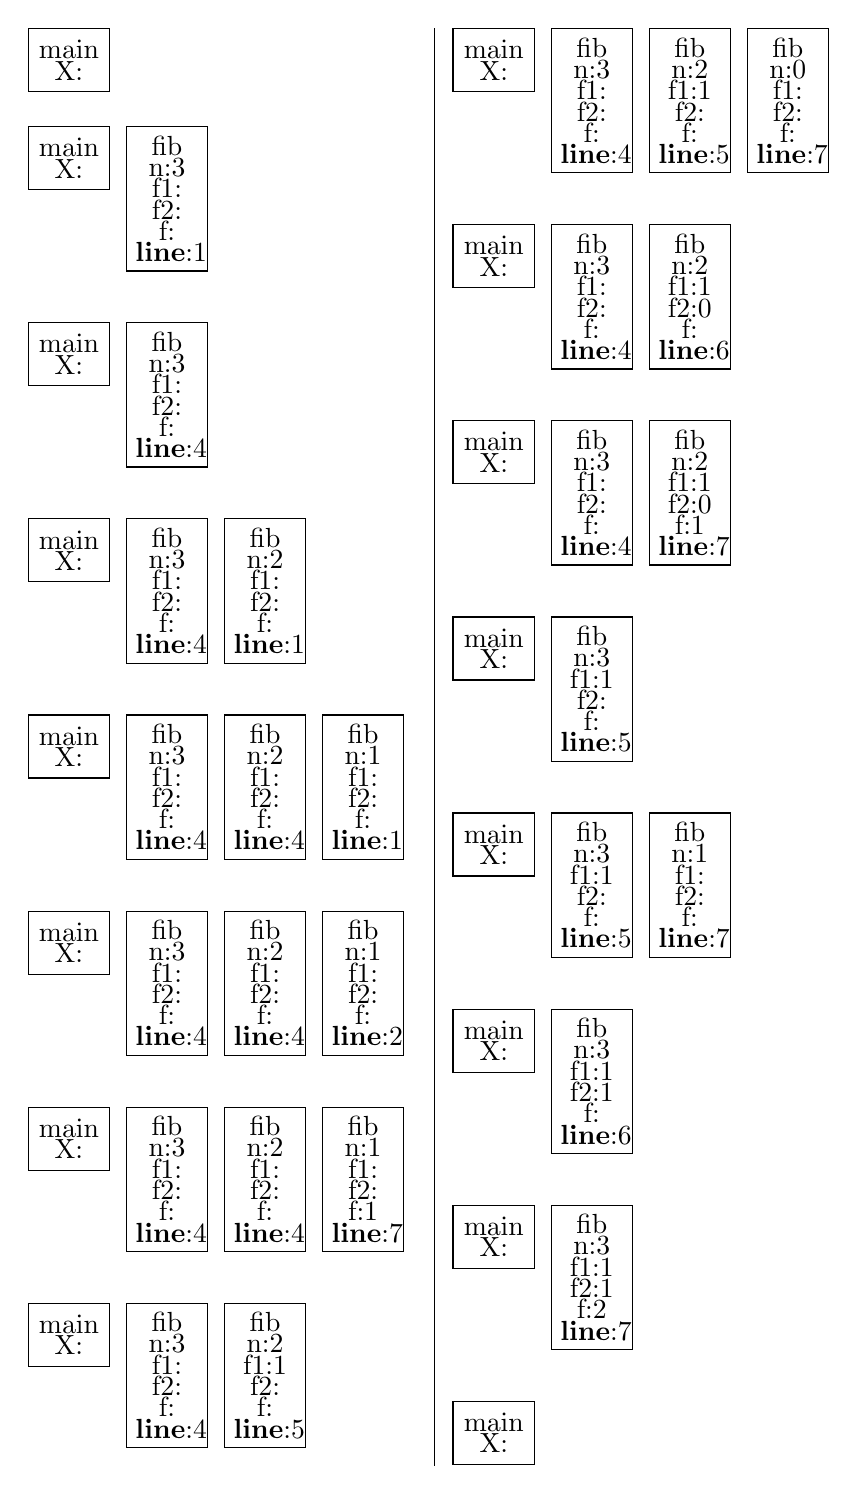
\begin{tikzpicture}[scale=0.83, place/.style={rectangle,draw, minimum size=8mm,text width=8mm,text centered, below}]
        \node   at ( 0, 0) [place] {main\\ \vspace{-1ex}X:};
        \node   at ( 0,-1.5) [place] {main\\  \vspace{-1ex}X:};
        \node   at ( 1.5,-1.5) [place]
            {fib\\ \vspace{-1ex}n:3\\ \vspace{-1ex}f1:\\ \vspace{-1ex}f2:\\ \vspace{-1ex}f:\\  \vspace{-1ex}\textbf{line}:1};

        \node   at ( 0,-1.5- 3.0*1) [place] {main\\  \vspace{-1ex}X:};
        \node   at ( 1.5,-1.5- 3.0*1) [place]
            {fib\\  \vspace{-1ex}n:3\\ \vspace{-1ex}f1:\\ \vspace{-1ex}f2:\\ \vspace{-1ex}f:\\  \vspace{-1ex}\textbf{line}:4};

        \node   at ( 0,-1.5- 3.0*2) [place] {main\\  \vspace{-1ex}X:};
        \node   at ( 1.5,-1.5- 3.0*2) [place]
            {fib\\  \vspace{-1ex}n:3\\ \vspace{-1ex}f1:\\ \vspace{-1ex}f2:\\ \vspace{-1ex}f:\\  \vspace{-1ex}\textbf{line}:4};
        \node   at ( 3,-1.5- 3.0*2) [place]
            {fib\\ \vspace{-1ex}n:2\\ \vspace{-1ex}f1:\\ \vspace{-1ex}f2:\\ \vspace{-1ex}f:\\  \vspace{-1ex}\textbf{line}:1};

        \node   at ( 0,-1.5- 3.0*3) [place] {main\\  \vspace{-1ex}X:};
        \node   at ( 1.5,-1.5- 3.0*3) [place]
            {fib\\  \vspace{-1ex}n:3\\ \vspace{-1ex}f1:\\ \vspace{-1ex}f2:\\ \vspace{-1ex}f:\\ \vspace{-1ex}\textbf{line}:4};
        \node   at ( 3,-1.5- 3.0*3) [place]
            {fib\\ \vspace{-1ex}n:2\\ \vspace{-1ex}f1:\\ \vspace{-1ex}f2:\\ \vspace{-1ex}f:\\  \vspace{-1ex}\textbf{line}:4};
        \node   at ( 4.5,-1.5- 3.0*3) [place]
            {fib\\ \vspace{-1ex}n:1\\ \vspace{-1ex}f1:\\ \vspace{-1ex}f2:\\ \vspace{-1ex}f:\\  \vspace{-1ex}\textbf{line}:1};

        \node   at ( 0,-13.5) [place] {main\\ \vspace{-1ex}X:};
        \node   at ( 1.5,-13.5) [place]
            {fib\\  \vspace{-1ex}n:3\\ \vspace{-1ex}f1:\\ \vspace{-1ex}f2:\\ \vspace{-1ex}f:\\  \vspace{-1ex}\textbf{line}:4};
        \node   at ( 3,-13.5) [place]
            {fib\\  \vspace{-1ex}n:2\\ \vspace{-1ex}f1:\\ \vspace{-1ex}f2:\\ \vspace{-1ex}f:\\  \vspace{-1ex}\textbf{line}:4};
        \node   at ( 4.5,-13.5) [place]
            {fib\\  \vspace{-1ex}n:1\\ \vspace{-1ex}f1:\\ \vspace{-1ex}f2:\\ \vspace{-1ex}f:\\  \vspace{-1ex}\textbf{line}:2};

        \node   at ( 0,-16.5) [place] {main\\  \vspace{-1ex}X:};
        \node   at ( 1.5,-16.5) [place]
            {fib\\  \vspace{-1ex}n:3\\ \vspace{-1ex}f1:\\ \vspace{-1ex}f2:\\ \vspace{-1ex}f:\\  \vspace{-1ex}\textbf{line}:4};
        \node   at ( 3,-16.5) [place]
            {fib\\  \vspace{-1ex}n:2\\ \vspace{-1ex}f1:\\ \vspace{-1ex}f2:\\ \vspace{-1ex}f:\\  \vspace{-1ex}\textbf{line}:4};
        \node   at ( 4.5,-16.5) [place]
            {fib\\  \vspace{-1ex}n:1\\ \vspace{-1ex}f1:\\ \vspace{-1ex}f2:\\ \vspace{-1ex}f:1\\  \vspace{-1ex}\textbf{line}:7};

        \node   at ( 0,-19.5) [place] {main\\ \vspace{-1ex}X:};
        \node   at ( 1.5,-19.5) [place]
            {fib\\ \vspace{-1ex}n:3\\ \vspace{-1ex}f1:\\ \vspace{-1ex}f2:\\ \vspace{-1ex}f:\\  \vspace{-1ex}\textbf{line}:4};
        \node   at ( 3,-19.5) [place]
            {fib\\  \vspace{-1ex}n:2\\ \vspace{-1ex}f1:1\\ \vspace{-1ex}f2:\\ \vspace{-1ex}f:\\  \vspace{-1ex}\textbf{line}:5};

        \draw (5.6, 0)--(5.6, -22);

        \node   at ( 6.5,0) [place] {main\\ \vspace{-1ex}X:};
        \node   at ( 8,0) [place]
            {fib\\  \vspace{-1ex}n:3\\ \vspace{-1ex}f1:\\ \vspace{-1ex}f2:\\ \vspace{-1ex}f:\\  \vspace{-1ex}\textbf{line}:4};
        \node   at ( 9.5,0) [place]
            {fib\\  \vspace{-1ex}n:2\\ \vspace{-1ex}f1:1\\ \vspace{-1ex}f2:\\ \vspace{-1ex}f:\\  \vspace{-1ex}\textbf{line}:5};
        \node   at ( 11,0) [place]
            {fib\\  \vspace{-1ex}n:0\\ \vspace{-1ex}f1:\\ \vspace{-1ex}f2:\\ \vspace{-1ex}f:\\  \vspace{-1ex}\textbf{line}:7};

        \node   at ( 6.5, -3) [place] {main\\ \vspace{-1ex}X:};
        \node   at ( 8, -3) [place]
            {fib\\  \vspace{-1ex}n:3\\ \vspace{-1ex}f1:\\ \vspace{-1ex}f2:\\ \vspace{-1ex}f:\\  \vspace{-1ex}\textbf{line}:4};
        \node   at ( 9.5,-3) [place]
            {fib\\  \vspace{-1ex}n:2\\ \vspace{-1ex}f1:1\\ \vspace{-1ex}f2:0\\ \vspace{-1ex}f:\\  \vspace{-1ex}\textbf{line}:6};

        \node   at ( 6.5,-6) [place] {main\\  \vspace{-1ex}X:};
        \node   at ( 8,-6) [place]
            {fib\\  \vspace{-1ex}n:3\\ \vspace{-1ex}f1:\\ \vspace{-1ex}f2:\\ \vspace{-1ex}f:\\  \vspace{-1ex}\textbf{line}:4};
        \node   at ( 9.5,-6) [place]
            {fib\\  \vspace{-1ex}n:2\\ \vspace{-1ex}f1:1\\ \vspace{-1ex}f2:0\\ \vspace{-1ex}f:1\\  \vspace{-1ex}\textbf{line}:7};

        \node   at ( 6.5,-9) [place] {main\\  \vspace{-1ex}X:};
        \node   at ( 8,-9) [place]
            {fib\\  \vspace{-1ex}n:3\\ \vspace{-1ex}f1:1\\ \vspace{-1ex}f2:\\ \vspace{-1ex}f:\\  \vspace{-1ex}\textbf{line}:5};

        \node   at ( 6.5,-12) [place] {main\\  \vspace{-1ex}X:};
        \node   at ( 8,-12) [place]
            {fib\\  \vspace{-1ex}n:3\\ \vspace{-1ex}f1:1\\ \vspace{-1ex}f2:\\ \vspace{-1ex}f:\\  \vspace{-1ex}\textbf{line}:5};
        \node   at ( 9.5,-12) [place]
            {fib\\  \vspace{-1ex}n:1\\ \vspace{-1ex}f1:\\ \vspace{-1ex}f2:\\ \vspace{-1ex}f:\\  \vspace{-1ex}\textbf{line}:7};

        \node   at ( 6.5,-15) [place] {main\\  \vspace{-1ex}X:};
        \node   at ( 8,-15) [place]
            {fib\\  \vspace{-1ex}n:3\\ \vspace{-1ex}f1:1\\ \vspace{-1ex}f2:1\\ \vspace{-1ex}f:\\  \vspace{-1ex}\textbf{line}:6};

        \node   at ( 6.5,-18) [place] {main\\  \vspace{-1ex}X:};
        \node   at ( 8,-18) [place]
            {fib\\  \vspace{-1ex}n:3\\ \vspace{-1ex}f1:1\\ \vspace{-1ex}f2:1\\ \vspace{-1ex}f:2\\  \vspace{-1ex}\textbf{line}:7};

        \node   at ( 6.5,-21) [place] {main\\  \vspace{-1ex}X:};
    \end{tikzpicture}
    \caption{fib函数的活动堆栈追踪:堆栈顶在右边。堆栈快照的序列排列在左列,再到右列。}
    \label{Fig:ActivationTraceOfFib}
\end{figure*}

\begin{example}\label{Example:3_1ActivationFrames}
Fibonacci数列的活动帧

图\ref{Fig:ActivationTraceOfFib}展示了当main函数执行x=fib(3)时,Fibonacci函数中
活动追踪的指针位置。fib的伪代码如下

\begin{lstlisting}[language={Java}, keywordstyle=\color{blue!70}, commentstyle=\color{red!50!green!50!blue!50}]
        int fib(int n)
        {
            int f, f1,f2;
        1:  if(n<2)
        2:      f=n;
        3:  else
            {
        4:      f1=fib(n-1);
        5:      f2=(fib(n-2);
        6:      f=f1+f2;
            }
        7:  return f;
        }
\end{lstlisting}

这段代码申明了一些局部变量,编译器通常为局部变量产生临时的空间,于是我们就
可以更细致的研究活动帧。事实上如同许多递归定义的函数一样,fib函数可以写成
一条“怪物”语句:
\begin{displaymath}
\mbox{\textbf{return}}\qquad n<2?n:fib(n-1)+fib(n-2);
\end{displaymath}
但是这种形式让我们追踪活动记录不是很方便。

图\ref{Fig:ActivationTraceOfFib}中左列顶行是在fib(3)调用之前帧堆栈,下一行
是fib进入之后帧堆栈。帧下面显示的行号是将要被执行的,如果帧不是帧堆栈顶部
的则行号是执行中的一行。程序的执行流总是在栈顶的活动帧"中",所以其他帧下面
的行号展示了在过程调用结束时执行流将到达的新的位置的堆栈帧。每一个局部变量
的值展示在冒号后面。没有值的变量则是还没有初始化。

随后的一行展示了执行到第4行,此时另一个函数调用发生。(就是说递归还没有
开始。)为了节约空间,下一行忽略了从1行到4行的过程,仅显示在下一个函数调用
之后的第4行。这次调用从2到7行,又一个同样的调用过程;f接受到值,这次调用将
返回。列的最后一行展示了前一次调用返回的是1;,返回值被存储到f1,第5行将被
执行。

右列的顶部展示了当函数调用fib(0)到达第7行的情形;它将返回了。fib(1)函数调用
产生的活动帧空间现在已经被复用了。接下来的3列展示了调用fib(2)的完成。它的
返回值被存储再调用fib(3)的活动帧中f1内。这个活动帧一直到第5行。下一个函数
调用再次扩展堆栈。之后堆栈就像前面一样重复工作了。

\end{example}

我们令一个\emph{简单语句}是一个过程中不再调用过程的语句。就像上面提到的fib
的代码,可以把过程写成每行一个过程调用或是简单语句的线性序列。假设每一个
简单语句运行常数时间,而且薄记一个函数调用的环境(设置下一个活动帧等)也是
常数时间。因此有:

\begin{lemma}\label{Lemma:3_1}
在不带\textbf{while}或\textbf{for}循环,但是可能有递归过程调用的计算过程中,
总的计算时间是$\Theta(C)$),这里C是在计算中过程调用的总数(包括作为
过程调用的函数)。
\end{lemma}

但是任意过程的规模$L$必须是自不变的;就是说不会因输入的不同而不同。在任意
固定算法中,对于算法中所有的过程都有一个最大的$L$。每一次运行算法的总时间,
确定是栈顶不同时间活动帧代表的过程调用的时间的总和。还可以合理的假定,由于
薄记工作的存在,每一个活动帧都会消耗时间,即使它是立即“返回”的。这些给
我们分析递归计算的运行时间的强有力工具。

\begin{theorem}
在不带\textbf{while}或\textbf{for}循环但是可能包含递归调用的计算中,
总的计算时间是$\Theta(C)$,这里C是在计算过程中调用的总数(包括作为
过程调用的函数)。
\end{theorem}

\begin{figure*}[!t]
    \centering
    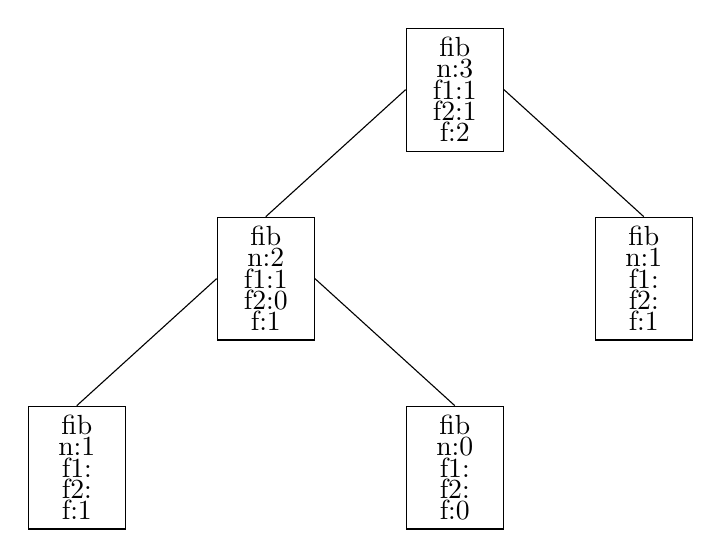
\begin{tikzpicture}[scale=0.8, place/.style={rectangle,draw, minimum size=10mm,text width=10mm,text centered, below}]
        \node (n1)  at ( 4,0) [place] {fib\\ \vspace{-1ex}n:3\\ \vspace{-1ex}f1:1\\ \vspace{-1ex}f2:1\\ \vspace{-1ex}f:2};
        \node (n2)  at ( 1,-3) [place] {fib\\ \vspace{-1ex}n:2\\ \vspace{-1ex}f1:1\\ \vspace{-1ex}f2:0\\ \vspace{-1ex}f:1};
        \node (n3)  at ( 7,-3) [place] {fib\\ \vspace{-1ex}n:1\\ \vspace{-1ex}f1:\\ \vspace{-1ex}f2:\\ \vspace{-1ex}f:1};
        \node (n4)  at ( -2,-6) [place] {fib\\ \vspace{-1ex}n:1\\ \vspace{-1ex}f1:\\ \vspace{-1ex}f2:\\ \vspace{-1ex}f:1};
        \node (n5)  at ( 4,-6) [place] {fib\\ \vspace{-1ex}n:0\\ \vspace{-1ex}f1:\\ \vspace{-1ex}f2:\\ \vspace{-1ex}f:0};

        \draw (n1.west) -- (n2.north);
        \draw (n1.east) -- (n3.north);
        \draw (n2.west) -- (n4.north);
        \draw (n2.east) -- (n5.north);
    \end{tikzpicture}
    \caption{fib(3)的活动树}
    \label{Fig:ActivationTreeOfFib}
\end{figure*}

进一步的,我们可以定义\emph{活动树(activation tree)}来作在算法一次运行
中所有过程调用的持久记录。每一个节点代表一个不同的过程调用,记录的位置
是在过程将要返回的那一点。根是算法的入口点。每一个节点的父节点是这个节点
创建时在帧堆栈顶部的那个节点。每一个节点的子节点从左到右是他们的活动帧
创建的顺序。图\ref{Fig:ActivationTreeOfFib}是个例子。

先序遍历活动树将是活动帧创建的顺序,树中节点的数量与执行时间是成比例的。
执行期间任何帧堆栈的快照都是对应树中的某条从根开始的线路。(在
\ref{Sec:Depth-firstSearchandRecursive}节的深度优先查找时我们回到这种
对应性)在\ref{Sec:WhyCanRecursiveTreeWork}小节中我们会检查活动树和
递归等式之间的关系。这对分析递归算法是很有帮助的。

\subsection{递归的提示-Method 99}\label{Sec:HintsForRecursionMethod99}
对于高级的算法开发,递归是一种必不可少的设计技术。对于递归的深层次的
讨论超出了本书的范围,但是这里有个小提示。可以参考本章后面的Notes和References
作进一步阅读。

确定一下你要编写的函数或过程要解决的问题的“度量单元”。然后假定你的task
只有一个过程叫做p,p可以处理\emph{0-100的规模}。这就意味着,设计解决方案的
时候你必须考虑至少100的规模--这就是你的“fantasy precondition”。

同样的,假定你可以调用一个给定的\emph{子例程},叫p99,它只做你的过程要做
的事情,有同样的函数原型,只是它的“fantasy precondition”是规模0到99。允许
你使用这个子例程(只要参数符合它的precondition),你不必写它的代码。

第二个线索是弄清楚你的程序非递归的情况。将非递归的情况弄到尽可能的小。你的
过程将总是从测试这种非递归情况开始,也叫做\emph{基本情况(base case)}。

最后的约定是决定p输入问题的规模刚好是100“too expensive”。(我们可以使
假想规模是1,000,000,000,但是method 999,999,999太长了。)但是将它的规模决定
成0或是更小的常量是完全可行的。

现在\emph{Method 99}指出了通过调用p99来写p的一种方法。(你不需要写p99,
所以不要想它。)当然,如果p是一个很简单的情况,则不需要调用p99。关键的一点是,
当p检测到问题不能立即解决的时候,它就需要创建一个子问题p99以解决之,
这满足下列3种情况:
\begin{enumerate}
\item 子问题的规模比p问题的规模小。
\item 子问题的规模比最小的规模要大(这里最小的规模是0)。
\item 子问题满足p99的其他preconditions(和p的precondition是一样的。)。
\end{enumerate}
在我们的假想中,子问题保证满足p99的规模约束(为什么?)。

如果你可以按这种方式分解问题,你就基本上解决了问题了。只是完成p的代码,
在需要的时候调用p99。

让我们实践一下写一个delete(L,x),就是从IntList中删除元素x,返回一个新的
包含所有L的元素但是不包含x的IntList。X也可能不包含在L中。
(\ref{Sec:ListADT}小节讨论了IntList ADT,他的cons是构造函数,first和
rest是存取函数,常量nil表示是空表。)

为了适用Method99, 我们假设我们只需要考虑list最多含有100个元素的情况,
而且我们有delete99可以使用。显然,如果我们可以从L中消除一个元素
(比如第一个),则我们可以让delete99去处理rest(L)。我们不知道rest(L)中
还有多少元素,但是我们采取了精明的实际的态度:如果L有100个元素,
则调用delete99就是ok的。如果超过100个是不会发生的(在我们的假想中)
我们仅假设delete只能处理100个元素或是更少的。

由于第二个线索,我们需要测试最坏的情况。什么是最坏的情况呢?既然允许x不
在L中,那么空表也是可能的。除了空表,还有一种情况需要马上解决而不需要
调用delete99:即x是L的第一个元素。在这种情况下,我们只需要简单的返回
rest(L)就完成了目标。

现在我们就用Method99来实现delete过程。
\begin{lstlisting}[language={Java},keywordstyle=\color{blue!70}, commentstyle=\color{red!50!green!50!blue!50}]
IntList delete(IntList L, int x)
{
    IntList newL, fixedL;
    if(L==nil)
        newL=L;
    else
        if(x==first(L))
            newL=rest(L);
        else
            fixedL= delete99(rest(L, x);
    newL= cons(fisrt(L, fixedL);
    return newL;
}
\end{lstlisting}
Ok,为了完成工作,只需要将子例程的99去掉,改成递归调用。

delete的过程也适合\emph{普通搜索例程}(参见定义\ref{Def:GeneralSearch}):
如果在没有数据就失败;如果这个数据搜索到了就成功(在上面的例子里是删除了);
否则继续搜索剩下的数据。


\subsection{递归过程的包装器}
经常的一个任务有一部分仅在开始或结束的时候做一次。在这种情况下,你需要将非递归
过程独立出来,再调用递归过程。我们称这个非递归过程是递归过程的包装器。有时候
包装器只是简单的初始化递归过程的参数。例如二分查找(算法\ref{Algo:BinrarySearch})
需要一个包装器使第一次递归有范围。包装器可能简单如下:
\begin{lstlisting}[language={Java},keywordstyle=\color{blue!70}, commentstyle=\color{red!50!green!50!blue!50}]
    int orderSearch(int[] E, int n, int k)
    {
        return binarySearch(E, 0, n-1, K);
    }
\end{lstlisting}


\section{什么是证明}\label{Sec:WhatIsTheProof}
再开始介绍证明之前,让我们对什么是证明做一个回顾。在\ref{Sec:LogicElement}小节
提到了,逻辑是一个规范化自然语言的系统,通过逻辑我们推理的更精确。证明是用逻辑
语句推理的\emph{结果}。本节描述详细的证明。实践中人们常忽略很多细节,将细节留
给读者去填充;这样的书写更精确的讲叫做\emph{证明框架}   。

定理、引理和推论都是可以被证明的语句,他们之间的区别并不是十分明显。一般来说,
人们对引理的兴趣不是它本身,引理的重要在于它能帮助证明人们感兴趣的命题,一般
称为定理。推论一般是定理的简单结果,但是并不是不重要。不管被证明的语句叫
“命题”、“定理”、“引理”、“推论”或是其他什么术语,证明过程是一样的。我们
将使用命题作为“一般性”的术语。

证明是符合逻辑规则的语句序列。每一个语句在形式语法层面上讲都是一个complete sentence:
它有一个主语和一个谓词,等等。尽管数学符号提供了一种缩写,但是语句还是
代表一个complete sentence。例如,“x=y+1”代表“x等于y+1”,这是一个完整的句子,
而“y+1”自己就不是一个句子。

这里精确的将逻辑语句组合成证明的inference rules可以无遗漏的列出来,我们将给出
比较多的非正式的规则。最重要的规则在\ref{Sec:LogicElement}小节给出,等式
\ref{Equa:ModusPonens}到\ref{Equa:RuleofCases}。每一个语句都可以从下面的事实得出新
的结论
\begin{itemize}
\item 众所周知的,且不是你将要证明的(例如,数学恒等式),或
\item 你要证明的定理的假定(前提),或
\item 在前面的证明中已经建立的语句(中间结论),或是
        item inductive hypothesis的实例,在\ref{Sec:PatternOfInductionProof}小节讨论
\end{itemize}
\noindent 证明的最后一个语句必须是要证明命题的结论。当一个证明分好几种情况时,
每一种情况度必须遵循上面的。

每一个语句不仅要给出新的结论,而且必须给出支持结论的事实。直接支持新结论的
语句称为新结论justification。含糊的justification是大多数逻辑错误的原因。

\subsubsection{定理或命题的格式}
你需要证明的命题有两个部分,\emph{假设}(也叫做\emph{前提premises}或\emph{hypotheses})
和结论。我们将结论称为目标语句。通常,命题有一个型如“对于集合W中所有的元素x”的部分,目标
语句是关于x的。(可能在语句中有几个类似x的变量。)实践中,集合W(世界的缩写)是
一族集合比如自然数、实数或是一族数据结构比如list、树、图。令要证明的命题有如下形式
\begin{equation}\label{Equ:3_1}
\forall x \in W[A(x)\Rightarrow C(x)]
\end{equation}
这里$A[x]$表示假设,而$C[x]$表示结论或叫做目标语句。符号$\Rightarrow$读作“蕴涵”。
方括号仅是为了更可读;他们和园括号一样。在自然语言中命题语句经常是这样的
形式“对于所有的$W$中的$x$,如果$A(x)$,则$C(x)$。”用词有各种变化。通常,我们
需要将大多数自然语句“揉”成一种向上面这样的标准形式,在我们要证明之前,我们需要
知道$x$,$W$,$A(x)$,$C(x)$分别代表什么。

\begin{example}\label{Example:3_2}
一个命题可能表示为:
\end{example}

\begin{proposition}
对于常数$\alpha<\beta$,$2^{\alpha n} \in o(2^{\beta n})$。
\end{proposition}
将其规范成等式\ref{Equ:3_1}的形式,
\begin{proposition}
对于所有$\alpha\in R$,对于所有$\beta\in R$,如果$\alpha$和$\beta$是常数
且$\alpha<\beta$,则$2^{\alpha n} \in o(2^{\beta n})$。
\end{proposition}

\noindent 让我们来检查两者的对应关系。显然二元组$(\alpha, \beta)$对应$x$,$R\times R$
对应$W$。引理的前提A(x)有3条语句:“$\alpha$是常数”,“$\beta$是常数”且“$\alpha<\beta$”。
结论C(x)是“$2^{\alpha n} \in o(2^{\beta n}$”。

\subsubsection{双列证明格式}
我们现在描述一种双列格式用于证明的表示。这种格式的目的是为了让证明中的
justifications更清晰;右列包含所有的justifications。每一个证明语句占用代行号的一行。
每一个在左边的\emph{新结论}它的justifications都在右边。引用前面已经证明的语句是通过它
的行号。

\begin{example}


例\ref{Example:3_2}的语句将用双列格式来证明。定理和证明都写的非常详细,作为一个证明中
如何写justifications的范例。我们包括所有的所有的证明者通常会期待读者自己填上的部分。

\end{example}

\begin{theorem}
对于所有$\alpha\in R$,对于所有$\beta\in R$,如果$\alpha$和$\beta$是常数
且$\alpha<\beta$,则$2^{\alpha n} \in o(2^{\beta n})$

\noindent 证明:

\begin{tabular}{ll}
\hline
语句  &Justification \\
\hline
1.首先我们想展示$\lim_{n\rightarrow \infty}\frac{2^{\beta n}}{2^{\alpha n}}=\infty$ & \\
2.$\frac{2^{\beta n}}{2^{\alpha n}}= 2^{(\beta-\alpha)n}$    &数学恒等式 \\
3.$\beta > \alpha$且都是常数  &定理的前提+数学恒等式\\
4.$\lim_{n\rightarrow \infty}2^{(\beta-\alpha)n} = \infty$ &(3)+已知的数学定理\\
5.$\lim_{n\rightarrow \infty}\frac{2^{\beta n}}{2^{\alpha n}} = \infty$ &(2)+(4)和带入\\
6.$2^{\alpha n} \in o(2^{\beta n}$  &(5)+$o$ 集合的定义(定义\ref{Def:LittleoAndomega})\\
\hline
\end{tabular}

\vspace{1ex}
几点注意事项:
\begin{enumerate}
\item 除了组成证明主题的语句,一般还包括一些“路线”或是“计划”语句来说明下面的
证明小段的目的,或是要使用的方法论,或是为了完成证明还需要的段落等等。

第一行就是一个\emph{计划}语句,不包含任何结论。因此它不能被后面的语句引用,它也不需要
justification。它告诉读者要成功证明的一个中间目标。这个目标在第5行完成。

\item 最后一行的新结论就是定理的目标语句。
\item 其他的所有行都被当作justification被引用了没有任何浪费。
\end{enumerate}

\end{theorem}

为了让证明完整、流畅,以双列格式写出一些结论的细节是一个很好的风格。通常完成
证明框架的细节是有益的,可以让你知道每一个新语句是怎么得出的。

\section{归纳证明}
归纳证明是证明一个关于无限个对象的集合的语句时的一种机制,通常也是唯一的机制。
我们这里描述的归纳方法通常叫做强归纳。强归纳是用于大多数关于算法和数据结构的
证明中最简单的形式。即使有时候不需要强归纳,但是使用使用强归纳也并不比使用它
的弱化版本要难。因此我们采用"one-size-fits-all"的原则,总是使用强归纳。

我们将会看到递归和归纳(强归纳)配合的非常完美。从大方面讲,证明是困难的,我们
需要尽可能的使得证明可理解,可靠精确。归纳证明和递归过程直接结构的类似性是在
证明复杂算法时的重要工具。

在大多数情况下归纳法是在自然数集合(非负整数,
\ref{Sec:AsymptoticOrderDefinitionAndSymbols}小节)或是正整数集合上。当然,归纳法
在更一般的集合也是有效的,只要他们提供两个属性:
\begin{enumerate}
\item 集合是部分有序的;就是说,在某些元素队上定义有顺序关系,但是可能并
        不是定义在所有的元素对上。
\item 集合中没有无限的降序元素链。
\end{enumerate}
例如,在\emph{所有整数}的集合上就不能使用归纳法。

\begin{figure*}[!t]
    \centering
    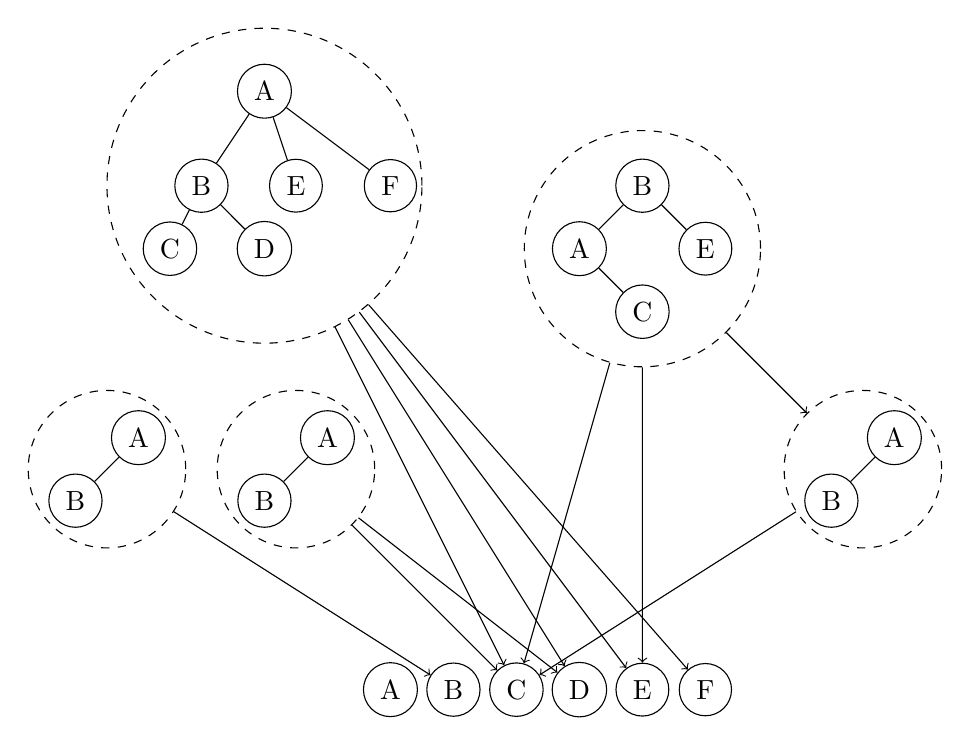
\begin{tikzpicture}[scale=0.8, place/.style={circle,draw, minimum size=5mm}]
        \node (A1)  at ( 1,0) [place] {A};
        \node (B1)  at ( 2,0) [place] {B};
        \node (C1)  at ( 3,0) [place] {C};
        \node (D1)  at ( 4,0) [place] {D};
        \node (E1)  at ( 5,0) [place] {E};
        \node (F1)  at ( 6,0) [place] {F};

        \node (X11) at (-3.5, 3.5) [place, minimum size=20mm, dash pattern=on 3pt off 3pt]{};
        \node (A21)  at ( -3,4) [place] {A};
        \node (B21)  at ( -4,3) [place] {B};
        \draw (A21)--(B21);
        \draw[->] (X11) --(B1);

        \node (X12) at (-0.5, 3.5) [place, minimum size=20mm, dash pattern=on 3pt off 3pt]{};
        \node (A22)  at ( 0,4) [place] {A};
        \node (B22)  at ( -1,3) [place] {B};
        \draw (A22)--(B22);
        \draw[->] (X12) --(C1);
        \draw[->] (X12) --(D1);

        \node (X13) at (8.5, 3.5) [place, minimum size=20mm, dash pattern=on 3pt off 3pt]{};
        \node (A23)  at ( 9,4) [place] {A};
        \node (B23)  at ( 8,3) [place] {B};
        \draw (A23)--(B23);
        \draw[->] (X13) --(C1);

        \node (A31) at (-1, 9.5) [place]{A};
        \node (B31) at (-2, 8) [place]{B};
        \node (C31) at (-2.5, 7) [place]{C};
        \node (D31) at (-1, 7) [place]{D};
        \node (E31) at (-0.5, 8) [place]{E};
        \node (F31) at (1, 8) [place]{F};
        \node (X1)  at (-1,8) [place, minimum size=40mm, dash pattern=on 3pt off 3pt] {};
        \draw (A31)--(B31);
        \draw (A31)--(E31);
        \draw (A31)--(F31);
        \draw (B31)--(C31);
        \draw (B31)--(D31);
        \draw[->] (X1) --(C1);
        \draw[->] (X1) --(D1);
        \draw[->] (X1) --(E1);
        \draw[->] (X1) --(F1);

        \node (B32) at (5, 8) [place]{B};
        \node (A32) at (4, 7) [place]{A};
        \node (E32) at (6, 7) [place]{E};
        \node (C32) at (5, 6) [place]{C};
        \node (X2)  at ( 5,7) [place, minimum size=30mm, dash pattern=on 3pt off 3pt] {};
        \draw (B32)--(A32);
        \draw (B32)--(E32);
        \draw (A32)--(C32);
        \draw[->] (X2) --(C1);
        \draw[->] (X2) --(E1);
        \draw[->] (X2) --(X13);
    \end{tikzpicture}
    \caption{展示的树的集合之间的\emph{subtree partial order}}
    \label{Fig:ExampleOfSubtreePartialOrder}
\end{figure*}

树就是一个部分有序的集合,经常对树使用归纳法。常用的部分顺序是:$t_1<t_2$,
当$t_1$是$t_2$的\emph{proper子树}时(参见图\ref{Fig:ExampleOfSubtreePartialOrder})。
后面我们将看到图有一个类似的部分顺序。在这样的集合上进行的归纳叫\emph{结构化归纳法}。

典型的需要归纳法来证明的定理包括:数学公式的定理、数据结构属性的
定理、递归等式的定理、这些经常在分析递归过程的运行时间时用到。
\ref{Sec:ProvingCorrectnessOfProcedures}节覆盖了那些需要证明过程完成了它的目标并会正确
的终止的定理。\ref{Sec:RecursiveEquation}节覆盖了典型的递归等式。

\subsection{归纳证明的模式}\label{Sec:PatternOfInductionProof}
归纳证明的第一件事就是:\\
\indent\emph{There is no such thing as "n+1" in an induction proof.}\\
不幸的是,很多读者学到了其他的。为什么我们把这个教条放在这里呢?

答案在我们早先给出的动机中--为了将递归和归纳联系起来。我们知道一个递归过程
是\emph{创建和解决小的子问题},再合并子问题来解决主要问题。我们希望我们的
递归证明也采用这个模式。对于证明来说,“主要问题”是要求的定理,而“子问题”是
要求的定理的小的实例,这些小的实例可以合并起来证明主要的实例。实践中,这些
小的实例差不多直接对应递归过程创建的精确的子问题。

所有的递归证明遵循一个通用的模式,我们称之为\emph{induction schema}。Schema
最关键的部分是\emph{inductive hypothesis}的正确引入。首先,我们给出一个证明
的例子,之后我们描述一般的schema,下面是几个例子。

\begin{example}
下面定理的证明展示了induction schema,在例子之后我们将描述其一般形式。
以\emph{宋体}表示的步骤几乎会出现在所有归纳证明的细节中。下面给出了证明
的细节,我们使用前面提到的双列证明格式。
\end{example}

\begin{proposition}
对于所有
$n \geq 0$,$\sum\limits_{i=1}^n = \frac{i(i+1)}{2} = \frac{n(n+1)(n+2)}{6}$ 。

\noindent 证明:

\begin{tabular}{ll}
\hline
语句  &Justification \\
\hline
1.\emph{证明归纳}n,来给出和的上限 & \\
2.\emph{基本情况是}n=0    & \\
3.此时等式的两边都等于0  &数学\\
4. \emph{对于$n>0$,假设} & \\
    $\sum\limits_{i=1}^n = \frac{i(i+1)}{2} = \frac{n(n+1)(n+2)}{6}$ \emph{对于所有$k\geq 0$且$k<n$成立} & \\
5.$\sum\limits_{i=1}^{n-1} = \frac{i(i+1)}{2} = \frac{(n-1)n(n+1}{6}$  &带入$k=n-1$\\
6.$\sum\limits_{i=1}^{n} = \sum\limits_{i=1}^{n-1}\frac{i(i+1)}{2}+\frac{n(n+1)}{2}$  &数学\\
7.$\sum\limits_{i=1}^{n} = \frac{(n-1)n(n+1)}{6} + \frac{n(n+1)}{2}$  &(5)+(6)\\
8.$\frac{(n-1)n(n+1)}{6} + \frac{n(n+1)}{2}= \frac{n(n+1)(n+2)}{6} $  &数学\\
9.$\sum\limits_{i=1}^n = \frac{i(i+1)}{2} = \frac{n(n+1)(n+2}{6}$ &(7)+(8)\\
\hline
\end{tabular}

\vspace{2ex}
一行一行的解释:
\begin{enumerate}
\item n是主要的归纳变量。注意命题的形式是$\forall n \in N[A(n)\Rightarrow C(n)]$。
        这里$A(n)$是简单true,而$C(n)$是等式。
\item 一个归纳证明始终有两种主要情况,称为\emph{基本情况}和\emph{归纳情况}。
        有时是基本情况s(复数)。
\item \emph{证明}基本情况s
\item 引入辅助变量$k$,进行递归假设。注意递归假设是$A(n)\Rightarrow C(n)$
        的形式,回到这个命题,$A(n)$仅仅是true;

        注意k的范围包括基本情况。

        注意k必须严格小于n;否则我们的假设就已经包括了我们要证明的。

        递归假设语句的标志着递归情况证明的开始。

\item 使用递归假设。(注意我们将“拉到n”。)辅助变量k在这里假设到了n-1。
        既然我们证明$n>0$的情况,k的这个值满足$0 \leq k<0$,就像在第4行要求的。

        辅助变量k可以在其他行假设到范围内的其他值。这是强归纳的一个好处。在这个
        简单的例子中,恰好不需要将k假设到别的值

\item Justification是一个标准数学等式,假设读者都知道。
\item Justification指出前面的两行支持这个新结论,但是不符合
        用到的\emph{推论规则},假设读者能指出来。
\item 采用了另一个数学等式。实际中,第6行到第9行可以合并成一行,假设
        读者可以指出这些步骤。但是,这样的浓缩可能导致许多错误的“证明”。
        证明者必须小心哪些精确的步骤需要写出来。

\item 结论恰好是目标语句$C(n)$。

\end{enumerate}

\end{proposition}

前面的证明遵循了一种模式,这种模式可以泛化成下面的schema。注意一般的术语,\emph{命题}
可以是\emph{定理}、\emph{引理}、\emph{推论}或是其他term,都不会改变证明过程。

\begin{definition}\label{Def:InductionProofSchema}
归纳证明模式

首先我们解释下面模式用到的符号。\emph{宋体}的内容重要表示重要的内容。在角括号
“<”“>”之间的条目是需要根据证明的命题来替换的。类似的,变量x和y也是根据命题
变化的。他们在集合W(world)之中。逻辑语句$C(x)$叫做\emph{目标语句}。逻辑语句$A(x)$
叫做\emph{命题假设}(或是假设s,如果它是一个合取式)。变量x叫做主要
归纳变量(或简称归纳变量)。变量y叫做辅助变量。

一个形如
\begin{displaymath}
\forall x \in W[A(x) \Rightarrow C(x)]
\end{displaymath}
的命题的归纳证明由下面的几部分组成。
\begin{enumerate}
\item \emph{证明是归纳x},<描述x>。
\item \emph{基本情况是(情况s是)}<基本情况>。
\item <\emph{证明}基本情况的目标语句,即带入基本情况,就是$C(base-case)$>。
\item \emph{对于}<X>\emph{大于}<基本情况>,假设对于所有的$y\in W$且$y<x$都有$[A(x)\Rightarrow C(x)]$。
\item <\emph{证明}目标语句,$C(x)$,就是命题出现的。>
\end{enumerate}
\end{definition}

一个归纳证明有两个主要情况:基本情况和递归情况。模式的第2步定义了基本情况;
第3步证明基本情况下定理成立。第4步定义了递归情况,而且使用了递归假设。
第5步证明递归情况下定理成立,这通常是证明的主要部分。$C(x)$的证明可以由下面部分支持:
\begin{enumerate}
\item x大于<基本情况>;
\item 命题的假设,$A(x)$ (不是$A(y)$);
\item 任意数量的归纳假设的实例,$[A(x)\Rightarrow C(x)]$,为辅助变量y带入严格小于x的W的元素。
\end{enumerate}
和普通的证明一样,证明中已经证明的结论,外部标识、定理都可以使用。

三个样板语句允许不带justification,因为他们没有给出任何结论;他们只是简单的
解释了证明的模式以及定义了一些符号。他们是
\begin{itemize}
\item “证明是归纳x…”
\item “基本情况是…”
\item “对于$x>$ <基本情况>,假设对于所有的$y<x$都有$[A(y)\Rightarrow C(y)]$。”
\end{itemize}
后两个语句将证明分成了两种情况:x是基本情况,x大于基本情况。两种情况必须
覆盖整个W,即覆盖所有x所有的范围。

\subsubsection{归纳模式的变体}
\begin{enumerate}
\item  如果假设$A(x)$并不实际依赖于x,则递归假设可以简化成:
        假设$C(x)$对于所有$y\in W$且y小于x都成立。你必须能解释
        why simplification is justified referring back to the
        justifications for proof statements.
\item 如果归纳需要多于一个的有次级情况,比如Fibonacci数列等式\ref{Equa:FibonacciSeries},
        可以有两个或多个基本情况。但是,最好仅引入归纳情况必须要的元素,因为每一个基本情况
        都需要它自己的证明。
\item 当归纳一个数据结构的时候比如list、tree、图或其他仅有部分顺序的集合,可以
        有多个基本情况元素。在图\ref{Fig:ExampleOfSubtreePartialOrder}中6个单个数是基本情况。
\end{enumerate}

\subsection{归纳证明一个递归过程}
下一个例子展示了归纳和递归是怎样一起工作的。我们将要证明的引理是关于一个
计算2-tree的external路径长度的过程的,这在底限分析中很有用
(参见\ref{Sec:LowerBoundOfAverageBehavior}小节)。
External路径长度在一些其他的问题中自然的被提出。首先我们需要一些定义。

\begin{definition}\label{Def:ExternalNodeAnd2_tree}
External节点和2-tree

二叉树基本类型中除了空树外的基本情况,是只有一个节点的树, 这个节点的类型
与树剩下节点的类型不同。这种节点叫external 节点。一个由\emph{external节点}
组成的树叫\emph{叶子},它没有任何子树了。其他节点的类型是\emph{internal节点},
它必须有两个孩子。这样的二叉树叫\emph{2-trees},因为每个节点要么有两个孩子,
要么没有。
\end{definition}

注意,如果我们将2-tree中所有的external节点替换成空树,则会剩下一个正常的,
不严格的二叉树。在2-tree中检查一个节点是否是叶子节点通常不需要判断这个节点
是否有孩子,因为叶子节点的类型与internal节点不一样。练习3.1展示了一个
2-tree的external节点必须比internal节点要至少多一个。

\begin{definition}
External路径长度

在2-tree树t中,t的\emph{external路径长度}是根到所有external节点路径长度的和。
路径的长度是路径的边数。可选的,2-tree的external路径长度可以递归定义如下:
\begin{enumerate}
\item 叶子的external路径长度是0。
\item 令t是一个非叶子节点,它有左子树L和右子树R(两者都可能是叶子)。
        t的 external 路径长度等于L的external路径长度+L的external节点数+R的
        external路径长度+R的external节点数。(t的external节点的数量是L和R
        的external节点数量的和。)
\end{enumerate}

两个定义的等价性是很显然的,因为每一条从t的根到L中的external节点的路径都比
从L的根到这个节点的路径要多1,R是类似的。
\end{definition}

\begin{figure*}[!t]
    \centering
    \begin{lstlisting}[language={Java}, keywordstyle=\color{blue!70}, commentstyle=\color{red!50!green!50!blue!50}]
        EplReturn calcEpl( TwoTree t)
        {
            EplReturn ansL, ansR;  // `子树返回的`
            EplReturn ans =new EplReturn(); // `要返回的`
        1.  if( t `是叶子`)
        2.      ans.epl=0; ans.extNum=1;
        3.  else
           {
        4.      ansL= calcEpl(leftSubtree(t));
        5.      ansR= calcEpl(rightSubtree(t));
        6.      ans.epl=ansL.epl+ ans.epl+
                        ansL.extNum+ ansR.extNum;
        7.      ans.extNum =ansL.extNum +ansR.extNum;
            }
        8.  return ans;
        }
    \end{lstlisting}
    \caption{计算2-tree external路径长度的函数。返回类型EplReturn是一个组织者类,用于函数返回2个值epl和extNum。}
    \label{Fig:LegthOf2-tree external}
\end{figure*}

\ref{Sec:BinaryTreeADT}小节的二叉树遍历框架可以简单的扩展成计算external路径长度。
参数的类型是TwoTree,其定义类似与BinTree,除了最小的树是叶子以外,BinTree的
最小树是空树。基本情况也要做相应的修改。函数需要返回两个值,所以我们需要
定义一个组织者类(参见\ref{Sec:OrganizerClass}小节),类名叫EplReturn,有两个
整数成员epl和extNum,分别表示external路径的长度和external节点的数目。我们看到函数
只是简单的实现了递归定义。我们现在能证明关于calEpl的引理。

\begin{lemma}\label{Lemma:ExternalNodeCount}
令t是任意2-tree。令epl和m分别是calcEpl(t)返回的epl和extReturn的值。则:
\begin{enumerate}
\item \emph{epl}是t的external路径的长度。
\item m是t的下external节点的数目
\item $epl \geq m\lg(m)$
\end{enumerate}

\emph{证明:} 在证明引理之前,让我们先把引理的语句和我们前面的证明模式关联起来,
等式\ref{Equ:3_1}。注意为了阅读把引理分成了几个句子。因此t是主要的递归变量
而W是所有2-tree的集合。第二个句子代表假设,所以表示$A(t)$。最后的三个结论组成$C(t)$。
和前面的例子一样,粗体表示了在任何递归证明中的关键部分。

\emph{证明是归纳}calcEpl的参数t,t with the "subtree" partial order。\emph{基本情况是}t
是叶子。到达calcEpl的第2行时,epl=0和m=1,这符合(1)(2),且 也符合(3)。

\emph{当}t不是叶子,\emph{假设引理对于所有s都成立},\emph{其中}s是t的严格子树。也就是
说,如果$epl_s$和$m_s$是calcEpl(s)返回的值,则$m_s$是s的external节点的数量,$epl_s$是
s的外部路径的长度,$epl_s\geq m_s\lg(m_s)$ 。令L和R分别表示t的左右子树。这里必须要求
是严格子树,因此可以采用递归假设。因为t是不是叶子,将执行从第4行到第7行的代码,则有
下面的等式
\begin{displaymath}
\begin{aligned}
    &epl= epl_L +epl_R + m_L +m_R\\
    &m=m_L+m_R
\end{aligned}
\end{displaymath}

通过递归假设和exteranl路径长度的递归定义,epl是t是exteranl路径长度。t的
每一个external节点都是同样是L或R的external节点,所以m是t的external节点的数目。

剩下的是证明 。我们注意到(参见练习3.2)函数$x\lg x$在$x>0$时是凸的,所以我们
可以使用引理\ref{Lemma:ConvexLemma1}。通过归纳假设我们有
\begin{displaymath}
\begin{aligned}
epl &\geq m_L\lg(m_L) +m_R\lg(m_R) +m\\
m_L\lg(m_L) + m_R\lg(m_R) &\geq 2(\frac{m_L+m_R}{2})\lg(\frac{m_L+m_R}{2})
\end{aligned}
\end{displaymath}
由于“$\geq$”的传递性,
\begin{displaymath}
epl \geq  m(\lg(m) -1) +m =m\lg(m)
\end{displaymath}
\end{lemma}

\begin{corollary}
一颗2-tree的external路径长度epl有底限:$epl \geq (n+1)\lg(n+1)$。

证明: 每一个有n个internal节点的2-tree都有(n+1)个external节点(参见练习3.1)采用
引理\ref{Lemma:ExternalNodeCount}。
\end{corollary}

经常发生递归过程需要用组织者类返回多个参数的情况,即使只需要一个量,但是返回
多个参数有利于简化程序。在这个例子里面,extNum不需要在查询,然是在递归过程中
返回它会极大的简化剩下的计算。对于其他的例子,参见练习3.13,这个练习要求你设计
一个函数来计算树顶点的独立集合的最大权。

\section{证明“过程”的正确性}\label{Sec:ProvingCorrectnessOfProcedures}
\emph{Things should be made as simple as possible-but not simpler.}\\
\indent\indent -Albert Einstein

一般认为证明一个程序的正确性试一个绝望的困难任务,\emph{一般的程序}。然而,证明
正确性对于解决问题和产生正确工作的程序来说是有价值的活动。诀窍是以已经证明为正确
的程序的风格去写程序。我们称之为证明友好风格。我们想证明应该是能帮助我们,而不是
成为额外的负担。让证明帮助我们的方法是以证明友好风格写程序,或者至少能在证明友好
风格和有效率的风格之间改变。

在这一节里面我们建立一套证明方法,从简单的开始逐渐复杂,但是一直会控制复杂的程度。
我们发展的风格将会用在这本书里面。基础是单赋值paradigm和递归。
单赋值paradigm在\ref{Sec:ParadigmOfSingleAssignment}小节引入。

\subsection{定义和术语}
\emph{Block}是一段代码,block有唯一的入口和唯一的出口。Blocks是程序代码和过程代码
的主要部分。一个\emph{过程}是一个带名字的block。过程常使用一些
\emph{参数(parameters)},以我们的理解来说,参数可以是\emph{输入}也可以\emph{输出}的。
为了简化问题,我们假设没有参数是既用于输入也用于输出;可以设计两个参数分别完成
输入和输出。还有,我们假设输入参数在过程执行过程中\emph{不会被修改}。如果需要修改,
将把参数复制到一个局部变量中。这个约定允许我们将输入参数当作postconditions without
 having to specify that we are referring to the values at the time of entry.

一个\emph{函数}是一个带输出参数的过程;如果有多个输出参数我们可以假设他们被封装在
一个\emph{组织者类}对象(参见\ref{Sec:OrganizerClass}节),因此他们可以被一个
\textbf{return}语句返回。因为仅有一个出口点,所以\textbf{return}语句必须是这个
出口点。这个形式允许我们将函数当作一个特殊的过程处理。

一个过程通常不引用\emph{非局部数据},即不在过程的头,也不在过程的体中定义的任何数据。
实际上,如果一个过程没有输出参数,调用它能产生效果的唯一方法是引用非局部数据。同样的,
过程可以定义局部数据。在过程执行的过程中,过程的参数也可以认为是一种局部数据。

一个在过程中的block也可以引用\emph{非局部数据},即在block之外定义的数据。这也叫做
全局数据。这可以是外层block封装的数据,或者是过程之外的数据,总之是符合使用的语言的
可见规则,能访问到的数据。

对于数组必须特别说明一下。如果将数组作为一个参数传递,数组的\emph{引用}被认为是局部
数据,但是数组的\emph{内容}被认为是非局部数据。类的的,在Java中,一个对象的\emph{引用}
是局部的,但是对象的\emph{实例域}是非局部的。更新非局部数据对于某些算法的效率非常重
要,但是为证明正确性带来了很大的麻烦。

\subsection{基本控制结构}\label{Sec:ElementaryControlStructures}
\begin{figure*}[!t]
    \centering
    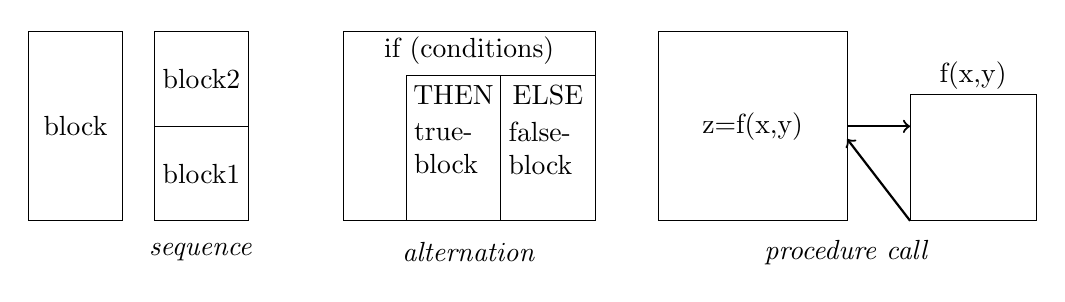
\begin{tikzpicture}[scale=0.8]
        \draw (0,0) rectangle (1.5,3);
        \node (P6)  at (0.75,1.5)  {block};
        \draw (2,0) rectangle (3.5,1.5);
        \node (P5)  at (2.75,0.75)  {block1};
        \draw (2,1.5) rectangle (3.5,3);
        \node (P4)  at (2.75,1.5+0.75)  {block2};

        \draw (5,0) rectangle (9,3);
        \node (P3)  at (7,2.7)  {if (conditions)};
        \draw (6,0) rectangle (7.5, 2.3);
        \node (P2)  at (6.75,2)  {THEN};
        \node (P2)  at (6.75,1.15)[text width=10mm]  {true-block};
        \draw (7.5,0) rectangle (9,2.3);
        \node (P1)  at (8.25,2)  {ELSE};
        \node (P2)  at (8.25,1.15)[text width=10mm]  {false-block};

        \draw (10,0) rectangle (13,3);
        \node (x43)  at (11.5,1.5)  {z=f(x,y)};
        \node (x3)  at (15,2.3)  {f(x,y)};
        \draw (14,0) rectangle (16,2);
        \draw [->, thick] (13, 1.5) -- (14, 1.5);
        \draw [->, thick] (14, 0) -- (13, 1.3);
        \node (P0)  at (2.75,-0.5)  {\emph{sequence}};
        \node (P0)  at (7,-0.5) {\emph{alternation}};
        \node (P0)  at (13,-0.5) {\emph{procedure call}};
    \end{tikzpicture}
    \caption{基本控制结构}
    \label{Fig:ElementaryProceduralControlStructures}
\end{figure*}


控制结构是导致不同的block被执行的机制。一开始我们仅考虑3种控制结构(参见
图\ref{Fig:ElementaryProceduralControlStructures}):\emph{顺序}(block1,
之后block2),\emph{选择}(if\emph{条件} then block1,else block2),和
\emph{过程调用}。在我们的基本证明方法学中省略\textbf{for}和\textbf{while}
循环是特意的。在发展出基本方法学之后,我们讨论3种构造的适应性
(在\ref{Sec:ProceduresWithLoop}小节)。

我们能不用循环写出任意可用的程序吗?吃惊的答案是"yes"。可以使用递归,,而且
用递归一般比用循环更简单。

“证明正确性”意味着证明一个过程的特定逻辑语句。例如“limited warranty”,statements
 are phrased carefully, so that sweeping that a proof would be hopelessly
difficult. 现在我们描述这些语句的形式。

\begin{definition}
Precondition, postcondition,和规范

\emph{Precondition}是一个关于输入参数和一个block(包括过程和函数)的局部数据的
逻辑语句,在block进入的时候,precondition应该是真。\emph{Postcondition}是一个
关于输入参数、输出参数、block的非局部数据的逻辑语句,在block退出的时候,
postcondition应该是真。Block的规范是preconditions和postconditions,
他们描述了block正确的行为。
\end{definition}

每一个block(包括过程和函数)必须有规范,如果我们想证明它的正确性的话。
为了证明正确的行为,证明下面形式的引理就足够了。

\begin{proposition}\label{Proposition:GeneralCorrectnessLemmaForm}
(通用正确性引理形式)如果当block进入的时候所有的\emph{preconditions}都满足,
则block退出的时候所有的\emph{postconditions}都应该是真。
\end{proposition}

假设一个block可以分为\emph{顺序结构}:block1 then block2。为了证明block的
正确性,证明如下形式的引理就足够了:

\begin{proposition}\label{Proposition:SequenceCorrectnessLemmaForm}
(顺序结构正确性引理形式)
\begin{enumerate}
\item Block的preconditions包含了block1的preconditions。
\item Block1的postconditions包含了block2的preconditions。
\item Block2的postconditions包含了block的postconditions。
\end{enumerate}
\end{proposition}

假设一个block可以分为\emph{选择结构}:if(\emph{condition})then true-block,
else false-block。为了证明block的正确性,证明如下形式的引理就足够了:

\begin{proposition}\label{Proposition:AlternationCorrectnessLemmaForm}
(选择结构正确性形式)
\begin{enumerate}
\item Block的preconditions逻辑与condtion为真包含了true-block的preconditions。
\item True-block的postcondition逻辑与condition为真(在true-block进入的时刻)包含了block的postcondition。
\item Block的preconditions逻辑与condtion为假包含了false-block的preconditions。
\item False-block的postcondition逻辑与condition为假(在false-block进入的时刻)包含了block的postcondition。
\end{enumerate}
\end{proposition}

\begin{figure*}[!t]
    \centering
    \subfloat{
    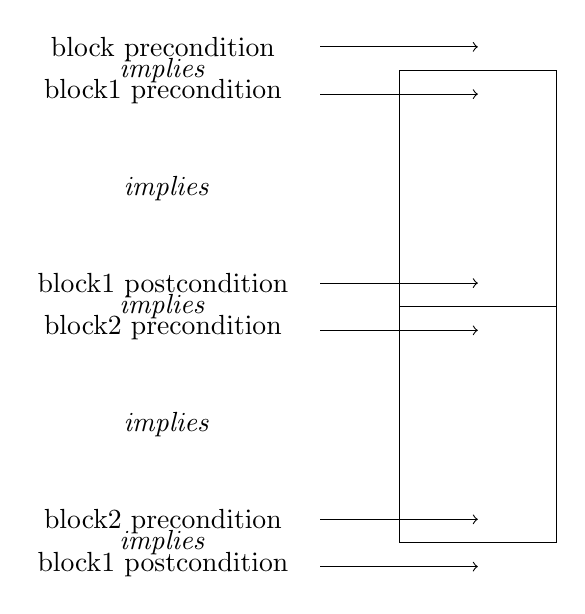
\begin{tikzpicture}[scale=1]
        \node  at (-1,6)[text centered, text width=32mm]
            {block precondition\\ \vspace{-1ex}\emph{implies}\\ \vspace{-1ex}block1 precondition};
        \node  at (-1,4.5)[text width=10mm]  {\emph{implies}};
        \node  at (-1,3)[text centered, text width=32mm]
            {block1 postcondition\\ \vspace{-1ex}\emph{implies}\\ \vspace{-1ex}block2 precondition};
        \node  at (-1,1.5)[text width=10mm]  {\emph{implies}};
        \node  at (-1,0)[text centered, text width=32mm]
            {block2 precondition\\ \vspace{-1ex}\emph{implies}\\ \vspace{-1ex}block1 postcondition};
        \draw (2,0) rectangle (4,3);
        \draw (2,3) rectangle (4,6);
        \draw [->] (1, 6.3) -- (3, 6.3);
        \draw [->] (1, 5.7) -- (3, 5.7);
        \draw [->] (1, 3.3) -- (3, 3.3);
        \draw [->] (1, 2.7) -- (3, 2.7);
        \draw [->] (1, 0.3) -- (3, 0.3);
        \draw [->] (1, -0.3) -- (3, -0.3);
    \end{tikzpicture}
    }
    \hfil
    \subfloat{
    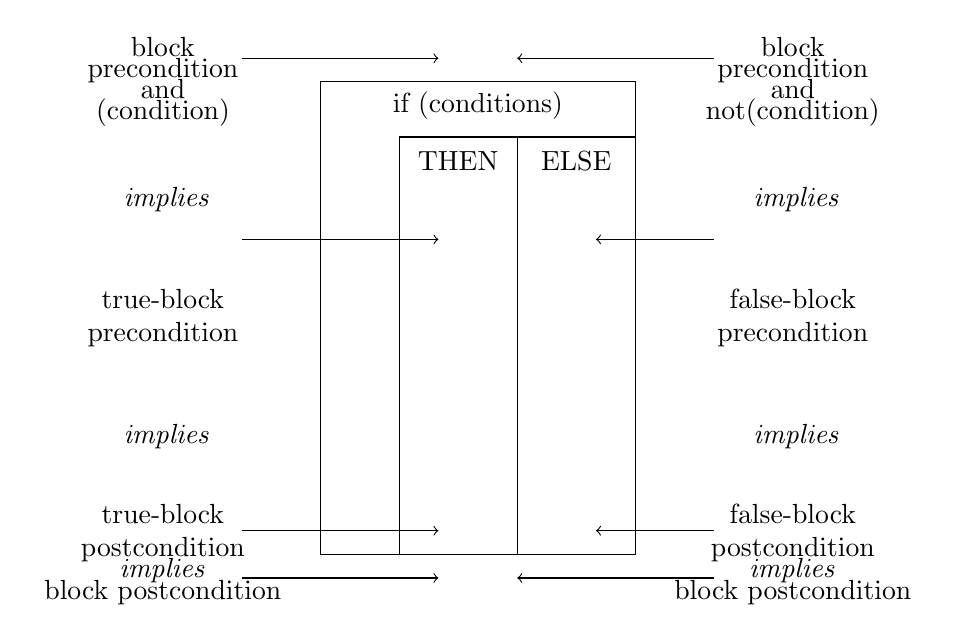
\begin{tikzpicture}[scale=1]
        \node  at (3,6)[text centered, text width=32mm]  {block\\ \vspace{-1ex}precondition\\ \vspace{-1ex}and\\ \vspace{-1ex}(condition)};
        \node  at (3,4.5)[text width=10mm]  {\emph{implies}};
        \node  at (3,3)[text centered, text width=32mm]  {true-block precondition};
        \node  at (3,1.5)[text width=10mm]  {\emph{implies}};
        \node  at (3,0)[text centered, text width=32mm]  {true-block postcondition\\ \vspace{-1ex}\emph{implies}\\ \vspace{-1ex}block postcondition};

        \draw (5,0) rectangle (9,6);
        \node at (7,5.7)  {if (conditions)};
        \draw (6,0) rectangle (7.5, 5.3);
        \node at (6.75, 5)  {THEN};
        \draw (7.5,0) rectangle (9,5.3);
        \node at (8.25,5)  {ELSE};

        \node  at (11,6)[text centered, text width=32mm]
            {block\\ \vspace{-1ex}precondition\\ \vspace{-1ex}and\\ \vspace{-1ex}not(condition)};
        \node  at (11,4.5)[text width=10mm]  {\emph{implies}};
        \node  at (11,3)[text centered, text width=32mm]  {false-block precondition};
        \node  at (11,1.5)[text width=10mm]  {\emph{implies}};
        \node  at (11,0)[text centered, text width=32mm]
          {false-block postcondition\\ \vspace{-1ex}\emph{implies}\\ \vspace{-1ex}block postcondition};

        \draw [->] (4, 6.3) -- (6.5, 6.3);
        \draw [->] (4, 4) -- (6.5, 4);
        \draw [->] (4, 0.3) -- (6.5, 0.3);
        \draw [->] (4, -0.3) -- (6.5, -0.3);
        \draw [->] (10, 6.3) -- (7.5, 6.3);
        \draw [->] (10, 4) -- (8.5, 4);
        \draw [->] (10, 0.3) -- (8.5, 0.3);
        \draw [->] (10, -0.3) -- (7.5, -0.3);
    \end{tikzpicture}
    }
    \caption{用来证明\emph{顺序}和\emph{选择}结构block的preconditions能推导出postconditions的推导链}
    \label{Fig:TheChainsOfInferences}
\end{figure*}

图\ref{Fig:TheChainsOfInferences}展示了命题\ref{Proposition:SequenceCorrectnessLemmaForm}
和\ref{Proposition:AlternationCorrectnessLemmaForm}是如何进行组合以获得类似
命题\ref{Proposition:GeneralCorrectnessLemmaForm}的证明形式的。

假设一个block由一个过程调用组成。为了证明block的正确性,证明如下形式的引理就足够了:
\begin{proposition}\label{Proposition:ProcedureCallCorrectnessLemmaForm}
(过程调用正确性引理形式)
\begin{enumerate}
\item Block的preconditions包含了以实际参数调用过程的preconditions。
\item Block的postconditions包含了以实际参数调用过程的postconditions。
\end{enumerate}
\end{proposition}

重要的是注意为了证明包含过程调用的block的正确性我们\emph{不}需要证明过程
调用本身的正确性;过程调用的正确性是单独的结果。

我们描述的证明的结构,这使得我们可以证明一个block的正确性,但是还没有
进入如何证明特定程序语句的细节。这是很有技术性和复杂的主题。

例如,假设我们看到java语句,“x=y+1”。在语句之后我们可以知道什么逻辑语句
(也就是什么是语句的postcondition)?似乎postcondtion是等式x=y+1。但是
假设语句是“y=y+1”?或是假设我们有一个语句序列“x=y+1, y=z”?

实践中,人们依赖“common sense” arguments,而不是正式的证明方法。不是试图
指出过程代码隐含什么逻辑语句,我们关注描述的postcondition是否能到达,而且
试图对于结论得出\emph{ad hoc arguments}。下一个主题讨论更好的方式。


\subsection{单赋值范例}\label{Sec:ParadigmOfSingleAssignment}
在早期对证明友好的编程风格的研究中,研究者发现引起证明困难的是主要是两种构造:
\emph{goto}语句和\emph{赋值}语句。消除赋值语句是不切实际的,所以早期的研究者
开始消除goto语句,结果导致了结构化编程的兴起。不幸的是,即使没有goto语句,
证明通常还是困难的。

最近,消除赋值语句的问题被重新提出,出的方法是消除重新赋值(overwriting)
赋值语句。就是说,在变量创建之后,变量只有一个值;一旦赋值之后就不能被覆盖。
既然,变量的值在变量的生存期之内不能改变,那么关于变量论证就简单了。
这就是\emph{单赋值范例}。

很多程序设计语言有一体化的单赋值范例约束,比如Prolog、ML、Haskell、Sisal
\footnote{for Streams and iteration in a single assignment language}
和SAC(单赋值C)。

在其他程序设计语言中,包括C、Fortran和Java,也可以在不改变程序的行为的情况
下转换成单赋值。这种转换用于编译优化和并行代码检测。研究发现采用单赋值形式
之后,程序分析可以达到很深的程度(参见本章后面的 Notes和References)我们能
在日常的编程利用单赋值范例的优点吗?

\emph{单赋值范例}不能通用,但是可以非常简单的用于非循环的局部变量。非循环代码包含
递归过程调用的代码,所以这个限制还不至于严重单赋值范例无用的地步。事实上,
Sisal的编译器将\textbf{for}和\textbf{while}循环转换成递归过程调用,所以它
能在转换后的程序中采用单赋值范例。由于强制使用了单赋值范例,Sisal编译器能
自动分析哪一段代码可以并行执行。但是,单赋值范例的限制形式也可以和
\textbf{while}和\textbf{for}循环一起使用。

复习一下本小节前面提到的使得证明变困难的赋值语句。在单赋值范例中“x=y+1;”
隐含等式x=y+1在整个程序中x有一个值。麻烦的语句是“y=y+1;”和“x=y+1; y=z”,
这两个违反单赋值范例的语句,将y第二次赋值了。

在没有循环的过程中,x和y可以是局部变量,我们总是可以通过定义额外的局部变量
做我们想做的计算。

\begin{example}\mbox{}\par
为了修正语句“y=y+1;”我们写“y1=y+1;”来代替,我们得到了有效的等式y1=y+1。
为了修正“x=y+1;y=z”我们必须有两个有效等式,x=y+1和y1=z。在两种情况中,过程
这个分支后面所有对y的引用都可以改成y1,因为y1是修改后的值。
\end{example}

让我们看一个更普通的困难:一个变量仅在选择结构一个的分支里面才更新,但是在
分支后面使用时混合了分支的两种情况。

\begin{example}\mbox{}\par
考虑下面的代码片段

\begin{lstlisting}[language={Java}, keywordstyle=\color{blue!70}, commentstyle=\color{red!50!green!50!blue!50}]
    1.if(y<0)
    2.  y=0;
    3.x=2*y;
\end{lstlisting}

根据我们前面说的,我们必须定义一个局部变量y1,然后将第二行替换成“y1=0”。但是
第3行呢?显然我们不知道该使用y还是y1。解决方案是:如果局部变量在选择结构的
一个分支里面赋值,则在所有的分支中赋以正确的值。在这种情况下,使用多条赋值语句
但是仅有一条赋值语句将会执行。修订后的符合单赋值范例的代码是
\begin{lstlisting}[language={Java}, keywordstyle=\color{blue!70}, commentstyle=\color{red!50!green!50!blue!50}]
    1.if(y<0)
    2.  y1=0;
    3.else
    4.  y1=y;
    5.x=2*y1;
\end{lstlisting}
现在我们对于变量有了一个清晰的逻辑关系($\Rightarrow$表示推导出,$\wedge$表示合取):
\begin{displaymath}
(y<0 \Rightarrow y1=0) \wedge (y\geq 0 \Rightarrow y1 =y )\wedge (x =2y1)
\end{displaymath}
创建额外变量的做法可能会导致效率下降,但是实际的编译器优化可以轻易的判断,如果
原来的y没有再被引用了它的空间用来存储y1。
\end{example}

然而,记住单赋值范例,虽然可以使用局部变量,但是对于有数组时是不适用的。需要更新
数组元素是很经常的事情,显然我们不能因为修改了一个元素就重新定义一个完整的数组。
即使我们这样做了,我们还是会在试图得到任何描述数组状态的逻辑语句时遇到困难。需要
更新对象的实例域时也会遇到同样的问题。

\subsubsection{转换没有循环的过程}
如果我们相对while或for循环采用本节讨论的证明工具,and the procedure is reasonably
compact,最简单的方法可能就是将循环转换成一个递归过程。

\begin{example}\mbox{}\par
算法\ref{Algo:SequentialSearch}给出了一个顺序查找的迭代过程。下面的代码给出
递归版本,并且使用单赋值范例。命题\ref{Proposition:GeneralCorrectnessLemmaForm}
到\ref{Proposition:AlternationCorrectnessLemmaForm}用于证明其正确性。(我们不
证明算法\ref{Algo:SequentialSearch}的正确性,它将一个变量赋予多个值导致了它的复杂。)
\end{example}

\begin{algorithm}\label{Algo:seqSearchRec}
顺序查找,递归

输入: E, m, num, K, 这里E是一个有num个元素的数组(索引从$0, \cdots, num-1$),K是
要查找的元素,$m \geq 0$是要查找的数组段的启示索引。为了简化,我们假定K和E的元素都
是整数,就和num一样。

输出:ans,一个在E中K的位置,范围是$m \leq ans <num$,或是-1,如果K在范围内没有找到的话。

注意:顶层调用必须是ans=seqSearchRec(E, 0, num, K)。

\begin{lstlisting}[language={Java}, keywordstyle=\color{blue!70}, commentstyle=\color{red!50!green!50!blue!50}]
    int seqSearchRec(int[] E, int m, int num, int K)
    {
        int ans;
    1.  if(m >= num)
    2.      ans=-1;
        else
        {
    3.      if( E[m]= =K)
    4.          ans=m;
    5.      else
    6.          ans= seqSearchRec(E, m+1m num, K);
        }
    7.  return ans;
    }
\end{lstlisting}

注意ans出现在三个赋值语句中,但是他们在不同的分支里面,所以这是符合单赋值范例的。
让我们来看看如何采用已知的命题来验证过程的正确性。

首先,我们需要公式化seqSearchRec的preconditions:
\begin{enumerate}
\item $m\geq 0$
\item 对于m≤i< num,E[i]是初始化的。
\end{enumerate}
现在我们给出目标或是postcondition,即在第7行必须是true的。
\begin{enumerate}
\item 如果$ans=-1$,则对于$m \leq j < num$, $E[i]\neq K$。
\item 如果$ans \neq -1$,则$m \leq  ans< num$,且$E[ans]=K$。
\end{enumerate}
现在,使用命题\ref{Proposition:GeneralCorrectnessLemmaForm},我们展示了如果当进入
seqSearchRec的时候precondition是满足的,则过程调用结束的时候postcondition就是
满足的。我们发现过程分离到三种选择情况中,第2,4,6行,最后汇聚到第7行的
return语句。命题\ref{Proposition:AlternationCorrectnessLemmaForm}用于每种情况。
对于每一个选择,导致选择的条件是可以用于证明每一个分支都导致postcondition的额外的信息。

如果到达第2行,则第1行的条件是true($m \geq num$)。第2行之后,ans= -1,之后就
到了第7行。此时,第1行条件为true包含了没有索引在范围$m \leq i < num$内,所以
条件1满足。条件2也是true,因为它的前提是false(复习\ref{Sec:LogicElement}小节)。

类似的,如果达到第4行,第1行的条件是false(所以m<num),且第3行的条件是true(E[m]=K)。
第4行自己建立了等式(ans=m)。合并这些域,条件2是正确的。等式($ans=m$)和precondition 1
可以得出postcondition 1的前提是false;因此postcondition 1是true。

最后,如果到达第6行,第1行和第3行的条件都是false(所以m<num$且E[m]\neq K$)。首先,我们
需要展示我们在第6行以实参“正确的调用”了seqSearchRec。就是说,当我们初始化这些实际
参数的时候,我们需要验证seqSearchRec的preconditions:
\begin{enumerate}
\item 如果$m \leq 0$,则$m+1 \leq 0$。
\item 范围$m+1, \cdots, num+1$包含在$m, \cdots, num-1$,所以E[i]是初始化的。
\end{enumerate}
现在,根据命题\ref{Proposition:ProcedureCallCorrectnessLemmaForm},我们可以得出结论
第6行的过程调用符合它的postconditions。既然第6行赋予ans的值就是调用返回的值,它
满足调用的postcondition(以实参m+1)。这些postconditions和参数$E[i]\neq K$隐含了
当前调用的postconditions(实参是m)。例如如果返回-1,隐含了$E[m+1], \cdots, E[num-1]$
都不包含K,所以$E[m], \cdots, E[num-1]$也不包含K。另外$ans \geq m+1$,也有$ans \geq m$。

因此我们展示了无论第7行如何到达,需要的postconditions都能达到。剩下的唯一问题是
是否存在可能性第7行永远无法到达,即进入了无限递归中。
\ref{Sec:TerminationOfRecursiveProcedures}小节讨论这个问题。
\end{algorithm}

练习3.6要求读者使用本小节的技术证明找两个整数最大公约数的欧几里得算法的正确性。

\subsection{带循环过程}\label{Sec:ProceduresWithLoop}
命题\ref{Proposition:GeneralCorrectnessLemmaForm}到
\ref{Proposition:ProcedureCallCorrectnessLemmaForm}给我们了一个在没有\textbf{for}
和\textbf{while}循环的情况下证明正确性的框架。只要有循环,单赋值范例通常就是不可能
的了,因为必须定义一个循环变量,indexed both by 过程中的行号和by number of passes
 through the loop to keep track of all the values taken on by the same 程序变量。
Then 必须小心的trace每一个变化中的历史值。我们相信相对于规格化过程本身来说,将
循环转换成递归过程在实践上更简单。

事实上,一旦我们理解了循环和递归版本之间的关系,通常没有必要实际的完成转换。
作为一个预处理步骤,我们必须下列:
\begin{enumerate}
\item 在循环体内部最宽范围内申明一个局部变量,遵循单赋值范例。就是说,在一轮仅给变量一个值。
\item 因为变量必须更新(而且必须声明在循环外面),在循环体的终结处做所有的更新。
\end{enumerate}
这些规则最小化了必须考虑到的不同情况的数量。

将一个\textbf{while}循环重新表示成递归的一般规则是:
\begin{enumerate}
\item 在循环内更新的变量变成一个过程的输入参数。他们在循环入口的初始值对应顶层
    递归调用的实际参数值。我们称这些为\emph{活动参数(active parameters)}.
\item 循环中引用的但是早先的定义的,
\end{enumerate}
for循环的规则类似。

\begin{figure*}[!t]
    \centering
    \begin{lstlisting}[language={Java}, keywordstyle=\color{blue!70}, commentstyle=\color{red!50!green!50!blue!50}]
    int factLoop(int n)
    {
        int k, f;
    1.  k=1;
    2.  f=1;
    3.  while(k<=n)
    4.  {
    5.     int fnew = f*k;
    6.     int knew= k+1;
    7.     k= knew; f=fnew;
    8.  }
    9.  return f;
    }

    int fact(int n)
    {
    9.   return factRec(n,1,1);
    }

    int factRec(int n, int k, int f)
    {
        int ans;
    3a. if(k>n)
    3b.    ans =f;
    4.  else
        {
    5.     int fnew = f*k;
    6.     int knew =k +l;
    7.     ans =factRec(n, knew, fnew);
        }
        return ans;
    }
    \end{lstlisting}
    \caption{while循环转换成递归函数。与转换不相关的花括号省略了。}
    \label{Fig:TransformationOfFactorialFunction}
\end{figure*}

在图\ref{Fig:TransformationOfFactorialFunction}中展示了一个结成函数的转换。
注意n是一个传递的参数。

除了第7行,factLoop的循环体是可以使用单赋值范例的。因此我们可以使用命题
\ref{Proposition:GeneralCorrectnessLemmaForm}到
\ref{Proposition:ProcedureCallCorrectnessLemmaForm}和变量之间的等式关系来思考
循环体,不牵涉到复杂的索引,也不需要处理通常碰到的一个变量在过程执行中有
不同的赋值。至少一直到第7行我们都可以使用单赋值范例的处理方法,此时变量的值
为下一轮“roll over”了。进一步的,如果我们能visualize这个“rolling over”作为
带新的实参的过程,并且这个过程有的\emph{比原来小的问题规模},我们就可以尝试
证明使用递归的算法形式。在这个有限的场景里面,单赋值范例可以用于带循环的过程。

\subsection{正确性证明作为调试工具}
证明正确性最大的实际价值——即使是非常不正式“心算”证明——在于证明能在编码和
测试没有开始之前就常常精确指出了bug所在。有时证明仅是完整的理顺一下过程的
preconditions和postconditions,并把他们作为注释写在代码中。(即使你的证明将是
一个“心算”,你也不应该逃避这步写文档的工作。)

许多程序bugs是过程的preconditions和调用过程时的实际条件不匹配,而且这种不匹配
是简单和显而易见的。另外大部分是因为postconditions不匹配。这种错误通常在考虑
命题\ref{Proposition:ProcedureCallCorrectnessLemmaForm}之后就会显而易见。

当问题比较微妙,一切看上“看上去都对”,你必须试图使用命题来为一个一个合适
大小的block来构在证明。这个过程就是问每一个block,“假设这个block完成了会怎样?”,
再问“它完成需要那些条件?”现在其一个block是否正确的达到这些要求?

如果代码中有一个bug,而且你推理的很小心,\emph{证明出错的地方就是bug的所在}。就是说,
bug就在两个block中穿过边界附近,在你发现postconditions和preconditions不匹配的地方。

例如,在递归顺序搜索(算法\ref{Algo:seqSearchRec})中,如果第1行的条件错写成了
($m \geq num-1$),则postcondition 1在第2行之后将不能得到,bug就定位了。

另一个例子,假设算法\ref{Algo:seqSearchRec}中1-2行和3-4行交换一下位置,就是说,
第1行变成“if(E[m]==k)”。我们给出的证明中所有提到的语句都重复行号上的变化,
但是过程有一个bug。为了在检查期间找出bug,我们必须注意到所有计算一个表达式的
语句的precondition是表达式中的所有数据元素都已经给出值,也就是我们不能access未
初始化的变量和实例域。如果m可能是大于num-1的数,我们不能保证这一点。再一次的,
证明试图暴露bug,但是仅在我们检查的很仔细的时候才行。在我们复查代码的时候问
一下“数据元素初始化了吗?”是一个很好的习惯。


\subsection{递归过程的终止}\label{Sec:TerminationOfRecursiveProcedures}
命题\ref{Proposition:GeneralCorrectnessLemmaForm}到\ref{Proposition:ProcedureCallCorrectnessLemmaForm},
\ref{Sec:ElementaryControlStructures}小节描述的引理等有递归过程的场合,展示
什么叫部分正确,因为他们没有给出过程是否该终止。为了完成完全正确的证明,
必须展示每一次递归调用都得到比原来要小的问题。

这时首先需要证明递归调用的precondition是满足的,其次是讨论传递给递归调用的
结构或是"问题规模"比调用者的要小。作为另一个正确性问题,实践中人们使用合理
的一般的讨论,而不用带公理和推论的正式的证明。

在许多情况下,问题的规模是一个非负整数,比如子范围的元素数量,链表中元素的数量,
诸如此类。例如在算法\ref{Algo:seqSearchRec}中,在
\ref{Sec:ElementaryControlStructures}小节“问题规模”方便的定义为n=(num-m),
未检查元素的数量。每次递归调用为导致减少1,最终会减少到0。

在有些情况下,问题的规模可以直接使用定义在结构上的partial order,通过一个输入
参数传递,比如\emph{subtree} partial order(参看图\ref{Fig:ExampleOfSubtreePartialOrder})。
例如,在一个二叉树遍历过程中,如图\ref{Fig:LegthOf2-tree external},如果
过程的输入参数是树T,而T不是基本情况,则T的子树比T“要小”in partial order。
因此在形式正确的二叉树结构上的递归过程会结束。

为了技术上的正确,在二叉树上做递归的过程必须有一个precondition,即输入参数T是
正确的二叉树--没有环。规范BinaryTree抽象数据结构类型一个动机(如同我们在
\ref{Sec:BinaryTreeADT}小节做的)是使得这个条件自动满足。

\subsection{二分查找的正确性}\label{Sec:CorrectnessofBinarySearch}
我们现在证明递归过程binarySearch的正确性(二分查找的细节参看
算法\ref{Algo:BinrarySearch})。这作为一个用归纳法证明递归过程的示范。一个
归纳证明建立在全部的不带循环递归过程正确性的基础之上;就是说,它建立在过程结束,
以及各它的preconditions蕴涵了postconditions的基础上。(如果递归过程调用
子例程,则子例程的正确性要在递归过程被证明之前作为一个假设添加。)

我们定义binarySearch的问题规模n= last -first+1,E在查找范围中的条目的数量。图
\ref{Fig:ProcedureforBinarySearch}只是为了方便做的一个重复。

\begin{lemma}
对于$n\geq 0$,如果\textbf{binarySearch(E, first, last, K)}被调用,问题的规模是
(last- first +1)=n,E[first], …, E[last]在非递减阶,则如果K不在E中first, …, last
的范围中返回-1,否则如果K=E[index]返回index。

证明  证明归纳n,问题的规模。基本情况是n=0。这时第1行是true,到达第2行,返回-1。

对于n>0,假设binarySearch(E, f, l,K)在$0\leq k <n$的问题规模k上满足引理,f和l是
任意索引满足$k=l-f+1$。因为$n>0$,第1行是false,$first \leq last$,流程到第4行,
然后是第5行。根据前面提到的不等式和等式$mid=\lfloor (first+last)/2\rfloor$,
得$first\leq mid \leq last$。因此mid在搜索范围内。如果第5行是true,过程在第6行
得到了结果。

现在假定第5行是false。从前面的两个不等式和n的定义,我们有(根据$\leq$的传递性)
\begin{displaymath}
\begin{aligned}
&(mid-1)-first+1 \leq (n-1)\\
&last-(mid-1)+1 \leq (n-1)
\end{aligned}
\end{displaymath}
所以对于第8行和第10行的两个递归调用递归假设都是适用的。

\begin{figure*}[!t]
    \centering
    \begin{lstlisting}[language={Java}, keywordstyle=\color{blue!70}, commentstyle=\color{red!50!green!50!blue!50}]
    int binarySearcha(int[] E, int first, int last, int K)
{
1   if( last< first)
2       index =-1;
3   else
    {
4       int mid = (first +last)/2;
5       if(K== E[mid])
6           index=mid;
7       else
        {
7           if(K<E[mid])
8               index= binarySearch(E, first, mid-1, K);
9           else
10              index= binarySearch(E, mid+1, last, K) ;
        }
11  return index;
}
    \end{lstlisting}
    \caption{binarySearch过程,算法\ref{Algo:BinrarySearch}的重复}
    \label{Fig:ProcedureforBinarySearch}
\end{figure*}

现在,如果第7行是true,则执行第8行。直接就可以发现binarySearch的precondition是满足
的,因为第8行的实际参数只有第3个参数改变了,而且是变小了。因此我们假定调用了完成
了binarySearch的目标。如果第8行的调用返回一个正的索引,这解决了当前了的问题。如果
第8行的调用返回-1,这意味着K不再E的范围$first, \cdots, mid-1$内。但是第7行隐含了K不在
范围$mid, \cdots, last$内,所以从当前的过程返回-1是正确的。如果第7行是false,则执行
第10行,是类似的。
\end{lemma}

关于证明需要强调的一点是,在我们(能)假定地8行和第10行的调用完成了他们的目标之前,
我们需要验证调用的preconditions。既然许多逻辑错误是由调用过程而没有满足过程
的precondition引起的,这种检查能揭示很多bugs。

\section{递归等式}\label{Sec:RecursiveEquation}
递归等式是定义在自然数上的函数,$T(n)$,它的值表达式中有一项或多项是小于n的整数的T。
换句话说,$T(n)$是归纳定义的。如所有的归纳一样,基本情况是单独定义,递归等式仅处理
比基本情况大的n。尽管我们的主要兴趣在用递归等式作为一种描述算法(运行时间,关键字
的比较次数,或者其他的重要工具)的函数式工具,但这不是递归等式唯一的用途。许多有趣
的数学函数可以用递归等式定义,比如Fibonacci数列,等式\ref{Equa:FibonacciSeries}。

用递归等式来描述递归过程是很自然的事情。本节的目的是展示如何从递归等式的代码中衍生
出递归等式,并描述算法中一些经常出现的patterns。\ref{Sec:RecursionTrees}节探索了如
何解一些常见的递归等式。因为不同资源的数量可能需要度量(时间,空间,关键字比较次数
等),我们将使用通用的术语\emph{cost}来给出递归等式的界限。

我们首先要指定一种度量方法来度量,需要解的递归过程的问题规模:令规模是n。递归等式
左边将是T(n)。为了构建递归等式的右边我们需要估计递归过程有多少不同的块,这些块
的cost与n的函数关系。经常有些块的cost是常数。We can just call all constants 1
if we are satisfied with an answer that is within a constant factor.

在我们的术语学中,\emph{子例程(subroutine)}是任意的过程,且不递归调用我们要分析
的过程;就是说,子例程中的调用序列不能有一个调用自己的。与子例程相关的数量一般带
角标S。与递归调用相关的数量一般带角标R。

如果过程没有循环,合并每一个块的最坏情况分析是简单的。
\begin{enumerate}
\item 对于块的\emph{序列},\emph{增加}单独的cost
\item 对于可选的块,包括基本情况,取选择项中\emph{最大的}。
\item 如果块包含子例程调用,指出实际参数与n的函数关系。为了简化问题,假设只需要
        一个参数规模,称为$n_s(n)$。我们需要知道子例程的cost函数$T_s$。则这个
        调用的的cost是$T_s(n_s(n))$。
\item 如果块包含递归调用,指出实际参数与n的函数关系,称为$n_r(n)$。则递归调用
        的cost是$T_r(n_r(n))$。这里的T与递归等式左边的一样。
\end{enumerate}
\noindent
等式右边出现的不含函数T(等式左边的)的部分称为\emph{非递归cost}。要把这个cost和
过程调用总的cost区分出来,过程总的cost也包含T。

合并块的平均行为分许需要区别的对待\emph{可选}的construct。对于所有可选项应该求
数学期望。Also,if the size of subproblems($n_r(n)$和$n_s(n)$)can vary for
different inputs,子例程的cost和递归调用的cost需要平均。由于这个原因,平均行为
分析通常认为比最坏情况分析要难。

\begin{example}\mbox{}\par
对于简单应用的规则,考虑算法\ref{Algo:seqSearchRec}的递归函数
seqSearchRec(E, m, num, K)

为了方便在这里重复一下:
\begin{lstlisting}[language={Java}, keywordstyle=\color{blue!70}, commentstyle=\color{red!50!green!50!blue!50}]
    1. if(m$\geq$num)
    2.  ans=-1;
    3.else if(E[m]==K)
    4.  ans=m;
    5.else
    6.  ans=seqSearchRec(E, m+1, num, K);
    7.return ans;
\end{lstlisting}

我们指定问题规模为要数组E的元素个数。因此n=num-m,这里m和num是当前调用的
第2个和第3个参数。让我们将过程分解为块,这样就可以采用规则了。块可以通过
行号的范围来描述。整个过程是1-7。可以参照下面的diagram,"OR"表示\emph{可选项},
";"表示\emph{序列}。

\begin{center}
    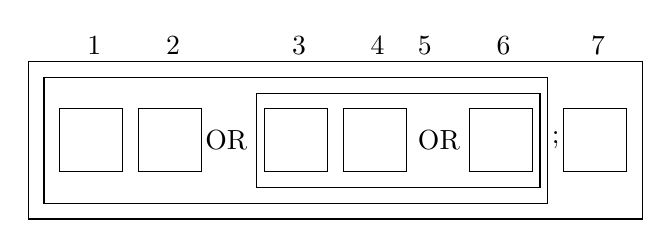
\begin{tikzpicture}[scale=1]
        \draw (-0.4,0) rectangle (7.4,2);
        \draw (-0.2,0.2) rectangle (6.2, 1.8);
        \node  at (0.4,2.2)[text width=1mm]  {1};
        \draw (0,0.6) rectangle (0.8, 1.4);
        \node  at (1.4,2.2)[text width=1mm]  {2};
        \draw (1,0.6) rectangle (1.8, 1.4);
        \node (P2)  at (1.9,1)[text width=1mm]  {OR};
        \draw (2.5,0.4) rectangle (6.1, 1.6);
        \node  at (3,2.2)[text width=1mm]  {3};
        \draw (2.6,0.6) rectangle (3.4, 1.4);
        \node  at (4,2.2)[text width=1mm]  {4};
        \draw (3.6,0.6) rectangle (4.4, 1.4);
        \node  at (4.6,2.2)[text width=1mm]  {5};
        \node (P1)  at (4.6,1)[text width=1mm]  {OR};
        \node  at (5.6,2.2)[text width=1mm]  {6};
        \draw (5.2,0.6) rectangle (6.0, 1.4);
        \node (P0)  at (6.3,1)[text width=1mm]  {;};
        \node  at (6.8 ,2.2)[text width=1mm]  {7};
        \draw (6.4,0.6) rectangle (7.2, 1.4);
    \end{tikzpicture}
\end{center}


基本情况是块2-2,基本情况需要排除在递归等式之外,递归等式只考虑非基本情况。
所有最里面的块s都是简单语句,除了6-6。当cost是运行时间时,我们假设简单语句
需要常量的运行时间,并用1代表任意常量时间(于是1+1=1)。当cost是某些特定操作
的数量时,则操作需要计数。For definiteness,我们将假设cost是数组元素比较的
次数。因此第3行cost是1,而在这个cost模型下其他简单语句没有cost。

注意算法\ref{Algo:seqSearchRec}中的第6行的调用,我们看到实际参数的第2个和
第3个是m+1和num,所以它的问题规模是num-(m+1)=m-1。所以,6-6的cost是T(n-1)。
整个块的cost由两部分构成,合并可选语句的最大项,合并序列块。块2-2作为一个
可选项被排除。注意1-7是1-6和7-7的和,给出seqSearchRec递归等式的右边
\end{example}

\begin{example}
对于其他例子,考虑二叉查找,算法\ref{Algo:BinrarySearch},在
\ref{Sec:CorrectnessofBinarySearch}小节有重复。问题规模是n=last-first+1。
消耗的度量是关键字比较,所以第5行消耗是1。第8行和第10行的递归调用的问题规模
是n/2和(n-1)/2,但是这是可选的,所以其合并的消耗取最大值,而不是两者的和。
剩下的语句中没有关键字比较,所以递归等式是
\begin{displaymath}
T(n)=T(m/2)+1
\end{displaymath}
在这个过程中,出现了两次递归调用实际上只有一次。在第4章我们将遇到排序过程,
有些排序中有两次递归调用,他们的递归等式的右边会有每一次递归调用代表的项。
\end{example}

如果规模$n_r(n)$或$n_s(n)$不是很清楚就有了新的问题。例如,在n个节点的二叉树
遍历中(\ref{Sec:BinaryTreeADT}小节),我们知道左子树和右子树总共有n-1个节点,
但是我们不知道两边各是多少。假设我们引入额外变量r表示右子树的规模。则我们
得到递归等式
\begin{displaymath}
T(n)=T(n-1-r)+T(r)+1, T(0)=1
\end{displaymath}
巧合的是,我们通过代入法能知道这个等式为$T(n)=2n+1$,即使我们不知道r。一般
我们没有这么幸运,而且对于不同的r可能结果不一样。这个问题在快速排序中就
出现了(\ref{Sec:AnalysisofQuickSort}小节)。


\subsubsection{普通递归等式}
我们能描述许多类递归等式,他们经常遇到且能通过标准方法解决(某种程度上)。
在所有情况下“子问题”指主要问题比较小的实例,需要递归解决的。符号b和c是常量。

\noindent
{\textbf{分而治之:}}在分而治之范例的许多情况中,子问题的大小是n/2或n乘以某个固定的比例。
例如我们已经看过的二分查找(\ref{Sec:SearchInOrderArray}节),我们在第
\ref{Sec:Chapter:Sort}章要学习的:归并(\ref{Sec:Mergesort}节)和
堆操作({Sec:FixHeap}小节)。使用\ref{Sec:Mergesort}节的归并作为例子,归并
排序做的比较数目是:
\begin{equation}\label{Equ:3_2}
T_{MS}(n)=T_{MS}(n/2)+T_{MS}(n/2)+M(n), T_{MS}(1)=0
\end{equation}
M(n)的消耗是归并子例程产生的。在我们能解决TMS(n)之前,我们需要知道M(n)是什么。

一般对于分而治之类型问题,规模n的主问题可以分解为b个($b \geq 1$)规模是n/c($c>1$)
的子问题。还有一部分非递归消耗$f(n)$(为了分解问题,且/或合并子问题的解到主问题)。

\begin{equation}\label{Equ:3_3}
T(n)=bT(\frac{n}{c})+f(n)
\end{equation}
我们称b是\emph{分支因子}。

{\textbf{Chip and Conquer:}}规模n的主问题可以“切掉一部分”成一个规模是n-c
的子问题($c>0$),再带一个$f(n)$的非递归消耗(为了分解问题,且/或合并子问题
的解到主问题)。
\begin{equation}\label{Equ:3_4}
T(n)=T(n-c)+f(n)
\end{equation}

{\textbf{Chip and Be Conquered:}}规模n的主问题可以“切掉一部分”成b个(b>1)
规模是n-c的子问题(c>0),再带一个f(n)的非递归消耗(为了分解问题,且/或合并子问题的解
到主问题)。我们称b是\emph{分支因子}。
\begin{equation}\label{Equ:3_5}
T(n)=bT(n-c)+f(n)
\end{equation}

如果子问题有不同的规模,但是所有的子问题规模都在n-cmax到n-cmin之间,责低限
可以分别使用$c_{max}$,$c_{min}$代替c来求。这种情况在练习3.11中考虑。

下一节我们探讨用数学方法分析这些典型的递归等式。

\section{递归树}\label{Sec:RecursionTrees}
递归树提供了一种分析我们已知递归等式的递归过程的消耗的工具(运行时间,关键字
比较次数或是其他测量方式)。首先我们将以一个例子展示如何从递归等式生成一个
递归树,然后我们将描述一般的过程。从一般过程中,我们将能派生出几种一般的
解决方案(引理3.14,引理3.15,定理3.15,定理3.17,等式3.12和3.13)。这些解决
方案覆盖许多实际算法分析中出现的递归等式,而且当遇到并不符合标准形式的递归等式
时,他们能作为一个粗略的guide。It is not necessary to follow all of the
technical details in this section to be able to apply the general solutions
mentioned.

每一个递归树的节点有两个域,\emph{size}和\emph{非递归cost域}。一个节点表示如下:

\begin{center}
\begin{tikzpicture}[scale=1,place/.style={rectangle,draw, fill=white,inner sep=0pt,minimum size=15mm}]
    \node (P6)  at (0,0) [place] {T(size)};
    \node (P5)  at (1.5,0) [place] {非递归cost};
\end{tikzpicture}
\end{center}

规模域代表这个节点处T的实际参数。我们加上递归名字T来提醒我们规模域不是cost。


\begin{example}\label{Example:3_10}
简单的分而治之的递归树

考虑递归等式:
\begin{displaymath}
T(n)=T(\frac{n}{2})+T(\frac{n}{2})+n
\end{displaymath}
这是等式\ref{Equ:3_3}的特殊情况,b=2和c=2。这是归并排序的一个稍微简单的形式,它
会在很多地方出现。我们将一步一步的构造出相应的递归树。第一步,是以辅助变量重
写等式(在递归假设中有一个类似的辅助变量),这有助于避免替换错误。我们称这个
递归等式为我们的\emph{工作拷贝}。

\begin{equation}\label{Equ:3_6}
T(k)=T(\frac{k}{2})+T(\frac{k}{2})+k
\end{equation}
只要节点的size域知道了一个节点就可以创建了;之后我们就可以用size域计算非
递归消耗的值。我们准备创建T(n)递归树的root节点;这里size=n。

\begin{center}
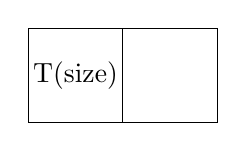
\begin{tikzpicture}[scale=1,place/.style={rectangle,draw, fill=white,inner sep=0pt,minimum size=12mm}]
    \node (P6)  at (0,0) [place] {T(size)};
    \node (P5)  at (1.2,0) [place] {};
\end{tikzpicture}
\end{center}
\end{example}

决定非递归cost域和没有完成孩子节点的过程叫扩展节点。我们将节点的规模域添上
准备扩展,这里是n,替换掉我们工作拷贝k,等式(3.6)。右边成为T(n/2)+T(n/2)+n。
所有带T的部分变成孩子节点,剩下的部分变成节点的非递归cost,如下
\begin{center}
    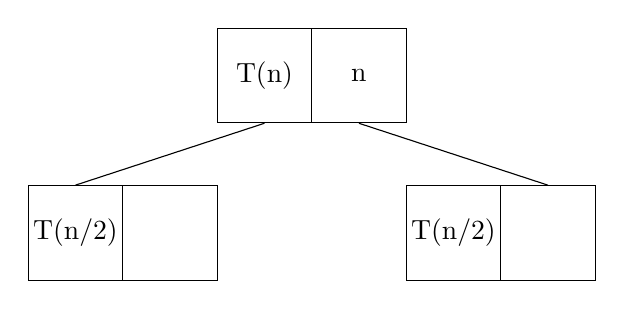
\begin{tikzpicture}[scale=1,place/.style={rectangle,draw, fill=white,inner sep=0pt,minimum size=12mm}]
    \node (P6)  at (0,0) [place] {T(n)};
    \node (P5)  at (1.2,0) [place] {n};
    \node (P4)  at (-2.4,-2) [place] {T(n/2)};
    \node (P3)  at (-1.2,-2) [place] {};
    \node (P2)  at (2.4,-2) [place] {T(n/2)};
    \node (P1)  at (3.6,-2) [place] {};

    \draw (P6.south)--(P4.north);
    \draw (P5.south)--(P1.north);
    \end{tikzpicture}
\end{center}

既然同样深度的所有节点看上去一样,我们可以在分支中产生他们。一般情况下,每一个
不完全节点必须根据自己的规模域产生。这里所有规模域都是n/2,所以我们用n/2代入
等式\ref{Equ:3_6}中的k,而且我们看到右边应该是T(n/4)+T(n/4)+n/2。所以现在我们有

\begin{center}

    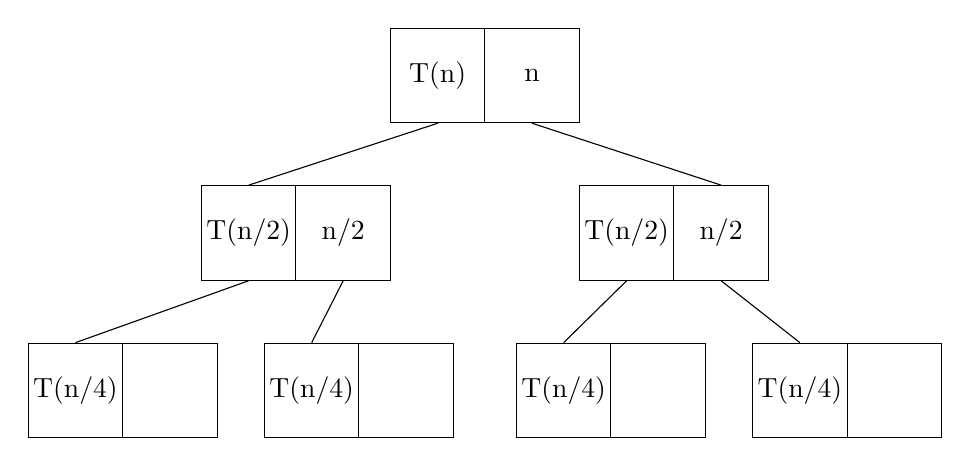
\begin{tikzpicture}[scale=1,place/.style={rectangle,draw, fill=white,inner sep=0pt,minimum size=12mm}]
    \node (P6)  at (0,0) [place] {T(n)};
    \node (P5)  at (1.2,0) [place] {n};
    \node (P4)  at (-2.4,-2) [place] {T(n/2)};
    \node (P3)  at (-1.2,-2) [place] {n/2};
    \node (P2)  at (2.4,-2) [place] {T(n/2)};
    \node (P1)  at (3.6,-2) [place] {n/2};

    \node (P41)  at (-4.6,-4) [place] {T(n/4)};
    \node (P31)  at (-3.4,-4) [place] {};
    \node (P21)  at (-1.6,-4) [place] {T(n/4)};
    \node (P11)  at (-0.4,-4) [place] {};
    \node (P42)  at (1.6,-4) [place] {T(n/4)};
    \node (P32)  at (2.8,-4) [place] {};
    \node (P22)  at (4.6,-4) [place] {T(n/4)};
    \node (P12)  at (5.8,-4) [place] {};

    \draw (P6.south)--(P4.north);
    \draw (P5.south)--(P1.north);
    \draw (P4.south)--(P41.north);
    \draw (P3.south)--(P21.north);
    \draw (P2.south)--(P42.north);
    \draw (P1.south)--(P22.north);
    \end{tikzpicture}

\end{center}

我们可以继续下一层,直到我们看出数的模式。图3.9展示了数扩展到另外一层;有8个
未完成孩子,其细节没有显示出来。这里我们可以看到以深度为函数的规模参数, n/2d,
非递归cost恰好也是n/2d。(复习下,为了方便,我们将根的深度定义为0)。在这个简单
的例子中,有同样数深度所有节点都是一致的,但是这不总是成立的。

我们在下一页总结生成一颗递归树的规则(s)。

\begin{figure*}[!t]
    \centering
    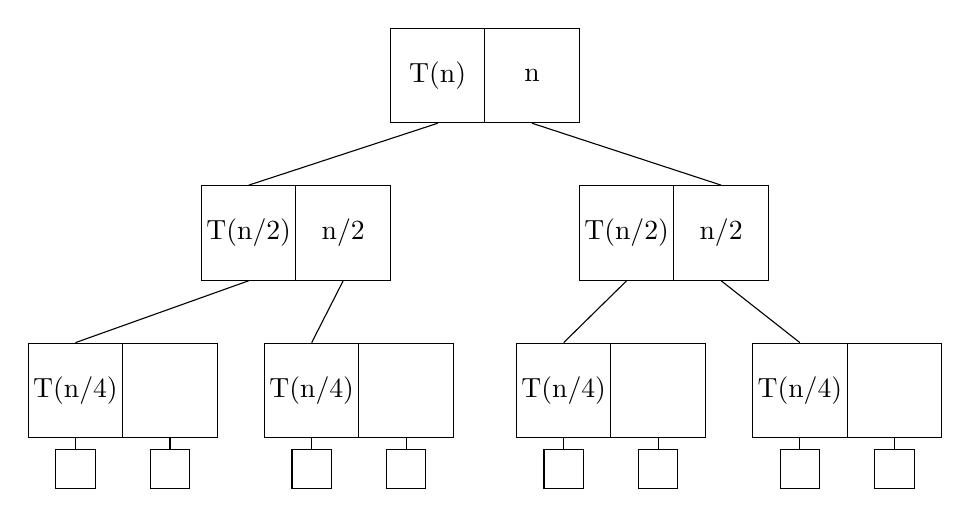
\begin{tikzpicture}[scale=1,place/.style={rectangle,draw, fill=white,inner sep=0pt,minimum size=12mm},
                            do/.style={rectangle,draw, fill=white,inner sep=0pt,minimum size=5mm}]
    \node (P6)  at (0,0) [place] {T(n)};
    \node (P5)  at (1.2,0) [place] {n};
    \node (P4)  at (-2.4,-2) [place] {T(n/2)};
    \node (P3)  at (-1.2,-2) [place] {n/2};
    \node (P2)  at (2.4,-2) [place] {T(n/2)};
    \node (P1)  at (3.6,-2) [place] {n/2};

    \node (P41)  at (-4.6,-4) [place] {T(n/4)};
    \node (P31)  at (-3.4,-4) [place] {};
    \node (P21)  at (-1.6,-4) [place] {T(n/4)};
    \node (P11)  at (-0.4,-4) [place] {};
    \node (P42)  at (1.6,-4) [place] {T(n/4)};
    \node (P32)  at (2.8,-4) [place] {};
    \node (P22)  at (4.6,-4) [place] {T(n/4)};
    \node (P12)  at (5.8,-4) [place] {};

    \node (P83)  at (-4.6,-5) [do] {};
    \node (P73)  at (-3.4,-5) [do] {};
    \node (P63)  at (-1.6,-5) [do] {};
    \node (P53)  at (-0.4,-5) [do] {};
    \node (P43)  at (1.6,-5) [do] {};
    \node (P33)  at (2.8,-5) [do] {};
    \node (P23)  at (4.6,-5) [do] {};
    \node (P13)  at (5.8,-5) [do] {};

    \draw (P6.south)--(P4.north);
    \draw (P5.south)--(P1.north);
    \draw (P4.south)--(P41.north);
    \draw (P3.south)--(P21.north);
    \draw (P2.south)--(P42.north);
    \draw (P1.south)--(P22.north);

    \draw (P41.south)--(P83.north);
    \draw (P31.south)--(P73.north);
    \draw (P21.south)--(P63.north);
    \draw (P11.south)--(P53.north);
    \draw (P42.south)--(P43.north);
    \draw (P32.south)--(P33.north);
    \draw (P22.south)--(P23.north);
    \draw (P12.south)--(P13.north);
    \end{tikzpicture}
    \caption{三层递归树。8个未完成孩子的规模域没有显示。}
    \label{Fig:BasicControlStructure}
\end{figure*}

\begin{definition}
递归树规则

\begin{enumerate}
\item 递归等式的\emph{工作拷贝}使用和原来不同的变量;称为辅助变量。这里令k是
    \emph{辅助变量}。原来递归等式的左边(假设是T(n))变成递归树根节点的规模域。
\item 一个未完成节点有一个规模域,但是没有非递归cost。
\item 决定给递归cost和未完成节点孩子的过程称为\emph{扩展}节点。我们取出待扩展节点
    的规模,代入递归等式的辅助变量k中。在右边包含T的部分变成节点的孩子;所有
    剩下的部分称为节点的非递归调用。
\item 扩展基本情况给出非递归调用,对于基本情况没有孩子。
\end{enumerate}
为了简化表示形式,我们假定递归等式的基本情况的cost不为0。如果等式的基本情况
的cost是0,我们可以只计算最小的不为0情况,将它作为基本情况。

事实上,我们经常假定基本情况cost是1,for definiteness。如果必要可以做变动。
\end{definition}

在任意递归树的子树里面,下面的等式成立:
\begin{equation}\label{Equ:3_7}
\mbox{根的规模}=\sum\mbox{扩展节点的非递归cost} + \sum\mbox{未完成节点的规模}
\end{equation}
这很容易由归纳法证明。在基本情况下,T(n)=T(n)。一次扩展后,根节点被扩展,
而孩子是未完成的,所以式\ref{Equ:3_7}给出的是原始的递归等式,以此类推。

\begin{example}
递归树

在例子\ref{Example:3_10}的7个节点递归树中(带4个未完成节点),式\ref{Equ:3_7}
表示为$T(n)=n+2(n/2)+4T(n/4)=2n+4T(n/4)$。
\end{example}

\begin{figure*}[!t]
    \centering
    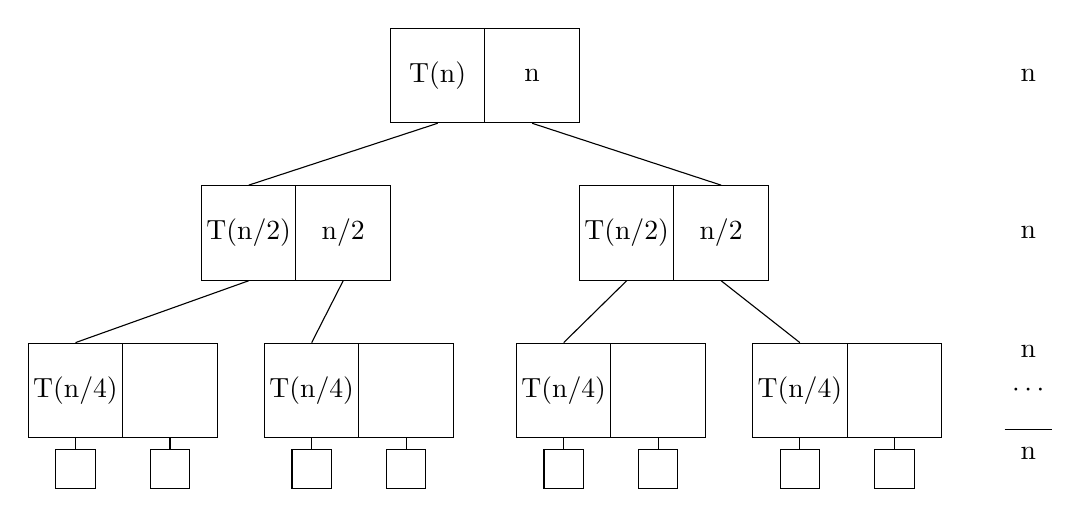
\begin{tikzpicture}[scale=1,place/.style={rectangle,draw, fill=white,inner sep=0pt,minimum size=12mm},
                            do/.style={rectangle,draw, fill=white,inner sep=0pt,minimum size=5mm}]
    \node (P6)  at (0,0) [place] {T(n)};
    \node (P5)  at (1.2,0) [place] {n};
    \node (P4)  at (-2.4,-2) [place] {T(n/2)};
    \node (P3)  at (-1.2,-2) [place] {n/2};
    \node (P2)  at (2.4,-2) [place] {T(n/2)};
    \node (P1)  at (3.6,-2) [place] {n/2};

    \node (P41)  at (-4.6,-4) [place] {T(n/4)};
    \node (P31)  at (-3.4,-4) [place] {};
    \node (P21)  at (-1.6,-4) [place] {T(n/4)};
    \node (P11)  at (-0.4,-4) [place] {};
    \node (P42)  at (1.6,-4) [place] {T(n/4)};
    \node (P32)  at (2.8,-4) [place] {};
    \node (P22)  at (4.6,-4) [place] {T(n/4)};
    \node (P12)  at (5.8,-4) [place] {};

    \node (P83)  at (-4.6,-5) [do] {};
    \node (P73)  at (-3.4,-5) [do] {};
    \node (P63)  at (-1.6,-5) [do] {};
    \node (P53)  at (-0.4,-5) [do] {};
    \node (P43)  at (1.6,-5) [do] {};
    \node (P33)  at (2.8,-5) [do] {};
    \node (P23)  at (4.6,-5) [do] {};
    \node (P13)  at (5.8,-5) [do] {};

    \draw (P6.south)--(P4.north);
    \draw (P5.south)--(P1.north);
    \draw (P4.south)--(P41.north);
    \draw (P3.south)--(P21.north);
    \draw (P2.south)--(P42.north);
    \draw (P1.south)--(P22.north);

    \draw (P41.south)--(P83.north);
    \draw (P31.south)--(P73.north);
    \draw (P21.south)--(P63.north);
    \draw (P11.south)--(P53.north);
    \draw (P42.south)--(P43.north);
    \draw (P32.south)--(P33.north);
    \draw (P22.south)--(P23.north);
    \draw (P12.south)--(P13.north);

    \node (Px1)  at (7.5,0)  {n};
    \node (Px2)  at (7.5,-2)  {n};
    \node (Px3)  at (7.5,-3.5)  {n};
    \node (Px4)  at (7.5,-4) {$\cdots$};
    \draw (7.2,-4.5)--(7.8, -4.5);
    \node (Px6)  at (7.5,-4.8)  {n};
    \end{tikzpicture}
    \caption{递归树中非递归cost的和。头3行的行和列在右边}
    \label{Fig:RowSumExample}
\end{figure*}

计算递归树的技术是:首先计算每一深度所有节点非递归cost的和;称为树这一层
的\emph{行和(row-sum)}。然后计算所有行和的和。继续图3.9的例子,有些行和已经
展示在图\ref{Fig:RowSumExample}中了。

为了计算行和的总和,(通常)需要知道递归树的最大深度。也就是规模约简
到基本情况的层数。

\begin{example}\label{Example:3_12}
递归树计算

对于例子\ref{Example:3_10}(参看图\ref{Fig:RowSumExample})我们观察规模与节点深度的
函数是$n/2^d$,所以基本情况发生在$d=\lg(n)$。既然每一行的和是n,树的
总和是$T(n)=n\log(n)$。
\end{example}

\subsection{分而治之, 一般情况}
使用例子\ref{Example:3_10}到例子\ref{Example:3_12}同样的步骤,我们能估计
一般分而治之递归等式(等式\ref{Equ:3_3},为了方便这里重复一下),以得到T(n)的渐进阶。
\begin{equation}\label{Equ:3_8}
T(n)=bT(\frac{n}{c})+f(n)
\end{equation}
这小节得到这种技术,但是引理和定理可以被理解,而且可以被单独使用。

首先,我们可以看到规模参数以因数c每次递减(我们令c=2为例)。因此基本情况
发生在$(n/c^D)=1$时,这里D是基本情况节点的深度。解方程得
$D=\lg(n)/\lg(c)\in \Theta(\log(n))$。然而,我们必须跳出所有深度
行和都一样的情况。

知道树\emph{有多少}叶子是很有用的。分支因数是b,所以深度D的节点数
是$L=b^D$。为了方便:$\lg(L)=D\lg(b)=(\lg(b)/\lg(c))\lg(n)$。系数
$lg(n)$经常出现,我们给它一个名字。

\begin{definition}\label{Def:CriticalExponent}
临界指数

对于等式\ref{Equ:3_3}中的b和c,我们定义临界指数为
\begin{displaymath}
E=\frac{\lg(b)}{\lg(c)}
\end{displaymath}
\end{definition}

通过引理\ref{Lemma:3_1},第8部分,对于E这样形式的对数可以使用任意方便的底,只要
分子分母同时还就行。以这个符号,有如下引理:

\begin{lemma}
等式\ref{Equ:3_8}递归树的叶子数量近似是$L=n^E$,这里E是定义
\ref{Def:CriticalExponent}中定义的临界指数。
\end{lemma}

假设叶子中的非递归cost是1,这告诉我们树的cost至少是nE。即使叶子的
非递归cost是0,在叶子的上层也肯定会有非0的cost的节点(或者极端情况下
叶子之上有常数层非0)。但是这层中仍然是$\Theta(n^E)$节点,所以保持的
$\Omega(n^E)$底限。

让我们总结下目前得到的结论。
\begin{lemma}\label{Lemma:3_15}
用前面使用的符号,我们近似有:

\begin{enumerate}
\item 递归树有深度$D=\lg(n)/\lg(c)$,所以有许多行和。
\item 第0层的行和是$f(n)$,即根的非递归cost。
\item 第D层行和是$n^E$,假设基本情况是1,或者$\Theta(n^E)$,in any event。
\item T(n)的值,也就是等式\ref{Equ:3_8}的解,是树中所有非递归cost的和,也就是所有行和的和。
\end{enumerate}
\end{lemma}

在许多实际情况中,行和形式是一个几何多项式(或者近似的上下界都是多项式)。
几何多项式的形式 (\ref{Sec:Calculous}小节)。常量r称为比率。Quit a few simplification occur
in practice that are based on the principle of 定理\ref{Theorem:1_13}的第2部分,which stated
that, for a 几何多项式 whose 比率不是1,the sum is in $\Theta$ of its largest term。
由这个定理和引理\ref{Lemma:3_15},我们可以得出结论:

\begin{theorem}\label{Theorem:LittleMasterTheorem}
(Little Master Theorem)以前面讨论的符号,和等式\ref{Equ:3_8}定义的T(n):

\begin{enumerate}
\item 如果行和组成了一个几何多项式(从第0行数的顶层开始),这里E是定义\ref{Def:InductionProofSchema}定义的
    临界指数。就是说,cost与递归树的叶子数量成比例。
\item 如果行和保持常量,$T(n)\in \Theta(f(n)\log(n))$。
\item 如果行和组成一个递减几何多项式,则$T(n)\in \Theta(f(n))$,这和根的cost成比例。
\end{enumerate}

\noindent{\emph{\textbf{证明}}} 在情况1中和由最后一项支配。在情况2中
有相当于$\Theta(\log(n))$的项。在情况3中和由最后一项支配。
\end{theorem}

为了更抽象适用范围更广,将这个定理泛化。泛化是很有用的,当等式\ref{Equ:3_8}中的函数
牵涉到对数时,因为之后行和可能不是很整洁。(对于更一般的版本,参见练习3.9。)

\begin{theorem}\label{Theorem:MasterTheorem}
(Master Theorem)以前面讨论的术语,递归等式的解

\begin{equation}
T(n)=bT(\frac{n}{c})+f(n)
\end{equation}
(重复等式\ref{Equ:3_3}和\ref{Equ:3_8})有如下解的形式,这里$E=\lg(b)/\lg(c)$是
定义\ref{Def:CriticalExponent}定义的临界指数。

\begin{enumerate}
\item 对于任意正数$\varepsilon$如果$f(n) \in Ο(n^{E-\varepsilon})$,则
    $T(n)\in\Theta(n^E)$,与递归树的叶子数量成比例。
\item 如果$f(n)\inΟ(n^E)$,则$T(n)\in\Theta(f(n)\log(n))$,as all node
    depths contribute about equally。
\item 对于任意正数$\varepsilon$如果$f(n)\in\Omega(n^{E-\varepsilon})$,并且
    对于$\sigma\geq\varepsilon$有$f(n)\inΟ(n^{E+\varepsilon})$,则$T(n)\in\Theta(f(n))$,
    与递归树根的的非递归cost成比例。
\end{enumerate}
(可能没有一种情况是适用的。)

\noindent{\emph{\textbf{证明}}} 深度d的节点有$b^d$个节点,每一个都有
非递归cost $f(n/c^d)$。因此我们对于等式\ref{Equ:3_8}的解有下面的通用表达式:
\begin{equation}
T(n)=\sum_{d=0}^{\lg(n)/lg(c)}b^df(\frac{n}{c^d})
\end{equation}
我们将只给出一个框架证明,它遵循定理\ref{Theorem:LittleMasterTheorem}给的理由。
(参看Notes和References有完全的证明)考虑情况3。忽略系数,对于某些正数$\varepsilon$,
f(n)关于$nE+\varepsilon$。所以
\begin{displaymath}
f(\frac{n}{c^d})\approx\frac{n^{E+\varepsilon}}{(c^d)^{E+\varepsilon}\approx\frac{f(n)}{c^{Ed+\varepsilon d}}}
\end{displaymath}
则$b^df(n/c^d)$是$f(n)b^d/(c^{Ed}c^{\varepsilon d})$。但是$c^E=b$,由于标准的标识符,
所以分母是$c^{Ed}$和分子$b^d$。我们最后有$f(n)/c^\varepsilon d$,给d一个递减
的几何多项式。其他情况的分析类似。
\end{theorem}

\subsection{Chip and Conquer,或者Be Conquered}
\begin{figure*}[!t]
    \centering
    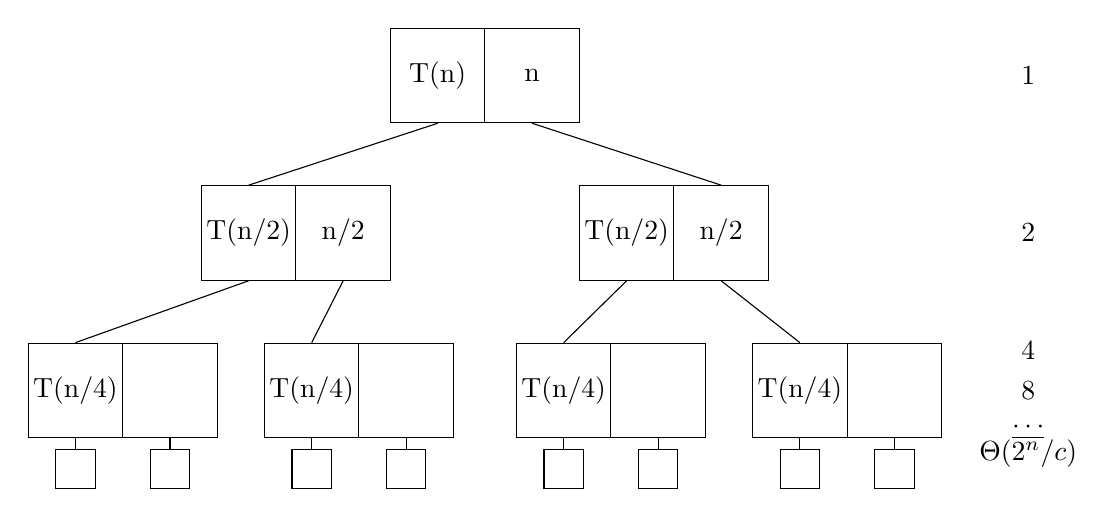
\begin{tikzpicture}[scale=1,place/.style={rectangle,draw, fill=white,inner sep=0pt,minimum size=12mm},
                            do/.style={rectangle,draw, fill=white,inner sep=0pt,minimum size=5mm}]
    \node (P6)  at (0,0) [place] {T(n)};
    \node (P5)  at (1.2,0) [place] {n};
    \node (P4)  at (-2.4,-2) [place] {T(n/2)};
    \node (P3)  at (-1.2,-2) [place] {n/2};
    \node (P2)  at (2.4,-2) [place] {T(n/2)};
    \node (P1)  at (3.6,-2) [place] {n/2};

    \node (P41)  at (-4.6,-4) [place] {T(n/4)};
    \node (P31)  at (-3.4,-4) [place] {};
    \node (P21)  at (-1.6,-4) [place] {T(n/4)};
    \node (P11)  at (-0.4,-4) [place] {};
    \node (P42)  at (1.6,-4) [place] {T(n/4)};
    \node (P32)  at (2.8,-4) [place] {};
    \node (P22)  at (4.6,-4) [place] {T(n/4)};
    \node (P12)  at (5.8,-4) [place] {};

    \node (P83)  at (-4.6,-5) [do] {};
    \node (P73)  at (-3.4,-5) [do] {};
    \node (P63)  at (-1.6,-5) [do] {};
    \node (P53)  at (-0.4,-5) [do] {};
    \node (P43)  at (1.6,-5) [do] {};
    \node (P33)  at (2.8,-5) [do] {};
    \node (P23)  at (4.6,-5) [do] {};
    \node (P13)  at (5.8,-5) [do] {};

    \draw (P6.south)--(P4.north);
    \draw (P5.south)--(P1.north);
    \draw (P4.south)--(P41.north);
    \draw (P3.south)--(P21.north);
    \draw (P2.south)--(P42.north);
    \draw (P1.south)--(P22.north);

    \draw (P41.south)--(P83.north);
    \draw (P31.south)--(P73.north);
    \draw (P21.south)--(P63.north);
    \draw (P11.south)--(P53.north);
    \draw (P42.south)--(P43.north);
    \draw (P32.south)--(P33.north);
    \draw (P22.south)--(P23.north);
    \draw (P12.south)--(P13.north);

    \node (Px1)  at (7.5,0)  {1};
    \node (Px2)  at (7.5,-2)  {2};
    \node (Px3)  at (7.5,-3.5)  {4};
    \node (Px5)  at (7.5,-4)  {8};
    \node (Px4)  at (7.5,-4.5) {\underline{$\cdots$}};

    \node (Px6)  at (7.5,-4.8)  {$\Theta(2^n/c)$};
    \end{tikzpicture}
    \caption{在一个chip-and-be-conquered 递归树的非递归cost的和。}
    \label{Fig:SummingNonrecursiveCosts}
\end{figure*}

一个不同的图片融合了等式\ref{Equ:3_4}和\ref{Equ:3_5}。如果分支因子大于1,我们
有等式\ref{Equ:3_5},这里为了方便重复一下:

\subsection{*为什么递归树能工作}\label{Sec:WhyCanRecursiveTreeWork}
这小结给出了一个给定递归等式和它的递归树的联系,以及编写好的用来计算
递归解的函数。读者可以略过本节,而不会丢失任何连续性。

一种可视化递归树的方式是想象我们实际上编写了一个简单的递归函数(称
为evalT(k))来计算递归等式的值,比如等式\ref{Equ:3_2}到等式\ref{Equ:3_5}。
这个函数的activation树非常精确的对应了递归树。递归等式看上去如
$T(k)=f(k)+\cdots $(带T的项)。我们假设我们的递归函数evalT有一个参数
k(代表问题规模),而一个局部变量nonrecCost来存储非递归cost的值
(也就是f(k))。忽略基本情况,假设evalT的
代码如下:
\indent   nonrecCost=f(k);
\indent   return nonrecCost+ … (带evalT的项)
这里带evalT的项只是模仿了递归等式右边带T的项。

递归等式的递归树,以T(n)为根,将是evalT(n)的activation树。(这假设
非递归cost函数f(k)可以用简单语句计算。\footnote{译注:即没有函数调用。})

可以看出,整个树的nonrecCost值得和就是顶层调用返回的值。我们假定顶层
调用时evalT(n),就是为了计算递归等式T(n)的值。
